%%%%%%%%%%%%%%%%%%%%%%%%%%%%%%%%%%%%%%%%%%%%%%%%%%%%%%%%%%%%%%%%%%%%%%%%%%%%
% AGUJournalTemplate.tex: this template file is for articles formatted with LaTeX
%
% This file includes commands and instructions
% given in the order necessary to produce a final output that will
% satisfy AGU requirements, including customized APA reference formatting.
%
% You may copy this file and give it your
% article name, and enter your text.
%
% guidelines and troubleshooting are here: 

%% To submit your paper:
\documentclass[draft]{agujournal2019}
\usepackage{url} %this package should fix any errors with URLs in refs.
\usepackage{lineno}
\usepackage[inline]{trackchanges} %for better track changes. finalnew option will compile document with changes incorporated.
\usepackage{soul}
\usepackage{wrapfig}
\usepackage{amsmath}


\linenumbers
%%%%%%%
% As of 2018 we recommend use of the TrackChanges package to mark revisions.
% The trackchanges package adds five new LaTeX commands:
%
%  \note[editor]{The note}
%  \annote[editor]{Text to annotate}{The note}
%  \add[editor]{Text to add}
%  \remove[editor]{Text to remove}
%  \change[editor]{Text to remove}{Text to add}
%
% complete documentation is here: http://trackchanges.sourceforge.net/
%%%%%%%

\draftfalse

%% Enter journal name below.
%% Choose from this list of Journals:
%
% JGR: Atmospheres
% JGR: Biogeosciences
% JGR: Earth Surface
% JGR: Oceans
% JGR: Planets
% JGR: Solid Earth
% JGR: Space Physics
% Global Biogeochemical Cycles
% Geophysical Research Letters
% Paleoceanography and Paleoclimatology
% Radio Science
% Reviews of Geophysics
% Tectonics
% Space Weather
% Water Resources Research
% Geochemistry, Geophysics, Geosystems
% Journal of Advances in Modeling Earth Systems (JAMES)
% Earth's Future
% Earth and Space Science
% Geohealth
%
% ie, \journalname{Water Resources Research}

\journalname{Enter journal name here}


\begin{document}

%%%%%%%%%%%%%%%%%%%%%%%%%%%%%%%%%%%%%%%%%%%%%%%
%  TITLE
%
% (A title should be specific, informative, and brief. Use
% abbreviations only if they are defined in the abstract. Titles that
% start with general keywords then specific terms are optimized in
% searches)
%
%%%%%%%%%%%%%%%%%%%%%%%%%%%%%%%%%%%%%%%%%%%%%%%

% Example: \title{This is a test title}

\title{=enter title here=}

%%%%%%%%%%%%%%%%%%%%%%%%%%%%%%%%%%%%%%%%%%%%%%%
%
%  AUTHORS AND AFFILIATIONS
%
%%%%%%%%%%%%%%%%%%%%%%%%%%%%%%%%%%%%%%%%%%%%%%%

% Authors are individuals who have significantly contributed to the
% research and preparation of the article. Group authors are allowed, if
% each author in the group is separately identified in an appendix.)

% List authors by first name or initial followed by last name and
% separated by commas. Use \affil{} to number affiliations, and
% \thanks{} for author notes.
% Additional author notes should be indicated with \thanks{} (for
% example, for current addresses).

% Example: \authors{A. B. Author\affil{1}\thanks{Current address, Antartica}, B. C. Author\affil{2,3}, and D. E.
% Author\affil{3,4}\thanks{Also funded by Monsanto.}}

\authors{=list all authors here=}


% \affiliation{1}{First Affiliation}
% \affiliation{2}{Second Affiliation}
% \affiliation{3}{Third Affiliation}
% \affiliation{4}{Fourth Affiliation}

\affiliation{=number=}{=Affiliation Address=}
%(repeat as many times as is necessary)


% Corresponding author mailing address and e-mail address:

% (include name and email addresses of the corresponding author.  More
% than one corresponding author is allowed in this LaTeX file and for
% publication; but only one corresponding author is allowed in our
% editorial system.)

% Example: \correspondingauthor{First and Last Name}{email@address.edu}

\correspondingauthor{=name=}{=email address=}



%%%%%%%%%%%%%%%%%%%%%%%%%%%%%%%%%%%%%%%%%%%%%%%
% KEY POINTS
%%%%%%%%%%%%%%%%%%%%%%%%%%%%%%%%%%%%%%%%%%%%%%%
%  List up to three key points (at least one is required)
%  Key Points summarize the main points and conclusions of the article
%  Each must be 140 characters or fewer with no special characters or punctuation and must be complete sentences

% Example:
% \begin{keypoints}
% \item	List up to three key points (at least one is required)
% \item	Key Points summarize the main points and conclusions of the article
% \item	Each must be 140 characters or fewer with no special characters or punctuation and must be complete sentences
% \end{keypoints}

\begin{keypoints}
\item enter point 1 here
\item enter point 2 here
\item enter point 3 here
\end{keypoints}

%%%%%%%%%%%%%%%%%%%%%%%%%%%%%%%%%%%%%%%%%%%%%%%
%
%  ABSTRACT and PLAIN LANGUAGE SUMMARY
%
% A good Abstract will begin with a short description of the problem
% being addressed, briefly describe the new data or analyses, then
% briefly states the main conclusion(s) and how they are supported and
% uncertainties.

% The Plain Language Summary should be written for a broad audience,
% including journalists and the science-interested public, that will not have 
% a background in your field.
%
% A Plain Language Summary is required in GRL, JGR: Planets, JGR: Biogeosciences,
% JGR: Oceans, G-Cubed, Reviews of Geophysics, and JAMES.
% see http://sharingscience.agu.org/creating-plain-language-summary/)
%
%%%%%%%%%%%%%%%%%%%%%%%%%%%%%%%%%%%%%%%%%%%%%%%

%% \begin{abstract} starts the second page

\begin{abstract}
[ enter your Abstract here ]
\end{abstract}

\section*{Plain Language Summary}
Enter your Plain Language Summary here or delete this section.
Here are instructions on writing a Plain Language Summary: 
https://www.agu.org/Share-and-Advocate/Share/Community/Plain-language-summary


%%%%%%%%%%%%%%%%%%%%%%%%%%%%%%%%%%%%%%%%%%%%%%%
%
%  BODY TEXT
%
%%%%%%%%%%%%%%%%%%%%%%%%%%%%%%%%%%%%%%%%%%%%%%%

%%% Suggested section heads:
% \section{Introduction}
%
% The main text should start with an introduction. Except for short
% manuscripts (such as comments and replies), the text should be divided
% into sections, each with its own heading.

% Headings should be sentence fragments and do not begin with a
% lowercase letter or number. Examples of good headings are:

% \section{Materials and Methods}
% Here is text on Materials and Methods.
%
% \subsection{A descriptive heading about methods}
% More about Methods.
%
% \section{Data} (Or section title might be a descriptive heading about data)
%
% \section{Results} (Or section title might be a descriptive heading about the
% results)
%
% \section{Conclusions}

\section{Introduction}\label{intro}
% examples of citation formatting: 
% \cite{Arthun2012}
% \citeA{Arthun2012}

% global context, why are we interested in the Arctic, Arctic Amplification; regional feedback mechanisms with sea ice loss, how does Arctic circulation, heat fluxes and water masses require use to understand transformation process
% FIGURE 1 to include: an Arctic map of Bathymetry or two of heat/freshwater content anomalies
% mean velocity of the Barents Sea AW layer to show the direction of flow
% start big, make this smaller and smaller until the Barents Sea
It is well-established that the Arctic is warming at a substantially faster rate than anywhere else on Earth in a process known as Arctic Amplification (AA) \cite{Manabe1980,Serreze2009,Cosimo2014,Huang2017,Rantanen2022}. This amplification results from several interrelated feedback mechanisms, though the relative contributions of each are still debated \cite{Pithan2014,Timmermans2018,Gong2017,Pistone2019,Previdi2021}. One important driver of AA is the rapid decline in winter sea ice extent and thickness \cite{Perovich2009,Dai2019}, closely linked to ocean heat transport and changes in surface heat forcing \cite{Onarheim2018,Stroeve2018,Oldenburg2024}. The implications of this amplification extend beyond the Arctic; warming in the lower troposphere over the Arctic can potentially influence mid-latitude weather patterns \cite{Honda2009,Petoukhov2010,Francis2012,Cohen2018,Coumou2018}. Along the inflow pathways from the Pacific and Atlantic, borealization—the process by which strengthened inflows of increasingly warm waters and sea ice retreat drive sub-Arctic regions to adopt features typical of southern boreal ecosystems—is altering species distributions and migratory patterns, with cascading effects on local economies and global biodiversity \cite{Fossheim2015,Polyakov2020_borealization,Ingvaldsen2021,Husson2024}. AA is not uniform, nor is the warming of the ocean explained by the changing atmosphere alone \cite{Marshall2014}. Winter sea ice decline and surface air temperature (SAT) amplification the highest globally in the Northern Barents sea, making it stand out as a focal point for Arctic change \cite{Screen2010,Onarheim2017,Isaksen2022,Rantanen2022}. For broader context, the full Arctic domain is shown in Figure~\ref{fig:wholeArctic}.

%\begin{figure}
\begin{wrapfigure}{l}{0.7\textwidth} % 'r' for right, '0.5\textwidth' for width

    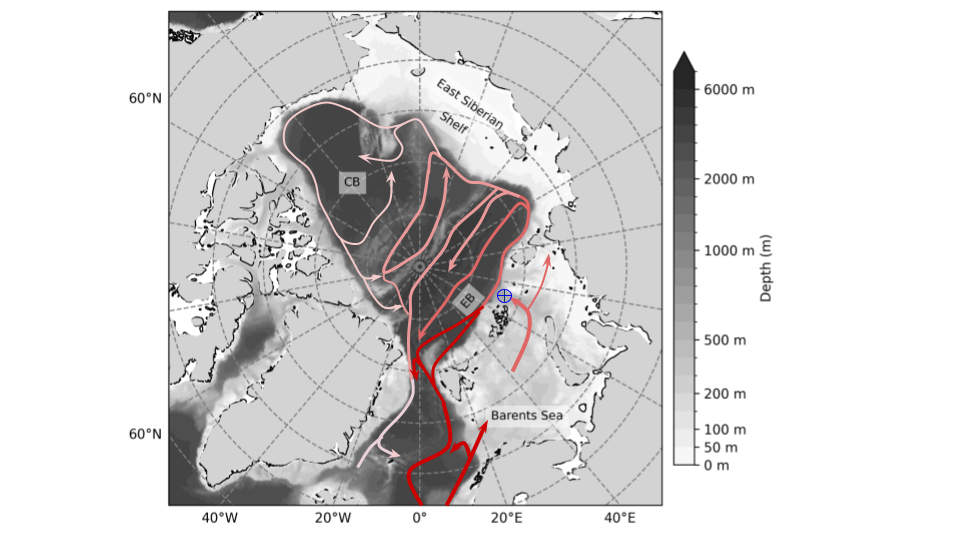
\includegraphics[width=\linewidth]{figs/Arctic_bathymetry.png}
    \caption{The bathymetry of the Arctic Ocean and marginal seas as represented in ASTE. Dashed gray lines show latitude and longitude and the depth of the seafloor is colored. Red arrows show the approximate path of AW as it loses heat around the Arctic.}
    \label{fig:wholeArctic}
    \vspace{-50pt}
\end{wrapfigure}


% what is happening in the Barents Sea and mechanisms causing this change
The Barents Sea has experienced a steady increase in heat content over recent decades \cite{Smedsrud2013,Bianco2024}, accompanied by a decline in near-surface freshwater content \cite{Watelet2020}. This can be visualized by the temperature and salinity profiles in Figure~\ref{fig:profiles}: the Southern part of the Barents Sea near the BSO has warmed and freshened, while the Northern part of the sea has exhibited warming and salinification over the time periods 2003--2007, 2008--2012, and 2013--2017. These changes are altering ocean stratification throughout the sea \cite{Lind2018,Hordoir2022}. The bathymetric features of the Barents Sea (Figure~\ref{fig:map}) play a key role in shaping these dynamics; the depth of the Bear Island Trench facilitates the greatest inflow of Atlantic-sourced water through the Barents Sea Opening (BSO) including the Svalbard Archipelago \cite{Kalhagen2024}, with other inflow North of Svalbard \cite{Lind2012,Lundesgaard2022}. The shallowness of the Sea as compared with the AO itself enhances the relative importance of atmospheric and surface processes, heat loss to the atmosphere modifies inflowing water \cite{arthun2010}, while the seasonal cycle of sea ice can brine to the surface layers of the sea \cite{schauer2002}. A key mechanism behind recent changes to the Barents Sea is the rapid sea ice reduction \cite{Rieke2023}, which can be attributed in part to the increased volume and warming of Atlantic inflow \cite{Smedsrud2010,Onarheim2018,Smedsrud2022}. This warm inflow and sea ice reduction reduces surface freshwater input, weakens stratification, and allows for enhanced vertical mixing, creating a feedback loop that accelerates "Atlantification": a term coined by \citeA{Polyakov2017} to describe the encroachment of Atlantic waters into the Arctic Ocean. While \citeA{Polyakov2017} primarily focused on the Eastern Arctic, the concept of Atlantification is also applicable to the Barents Sea, where similar processes are transforming it into a warm, well-mixed Atlantic structure \cite{Arthun2012,Gerland2023}. During winter, when surface heat fluxes are negative, ocean heat transport (OHT) from the Atlantic inflow is the dominant cause of ice melt \cite{Ivanov2012,Tsubouchi2021}, increasing the ice-free area and amplifying surface heat release \cite{Skagseth2020}. The northward spread of warm, saline water \cite{Oziel2016} changes local ecologies \cite{Bogstad2015,Dalpadado2014,Ingvaldsen2021} and further erodes stratification \cite{Lind2018}. This warm water cools along its inflow path, but the ability of the Barents Sea to cool Atlantic inflow appears to be diminishing \cite{Shu2021,Skagseth2020}. These interlinked feedbacks--sea ice loss, atmospheric changes due to AA, and OHT--remain complex, and understanding their interactions is critical for predicting the future regimes of the region.

\begin{wrapfigure}{l}{0.6\textwidth} % 'r' for right, '0.5\textwidth' for width
    \centering
    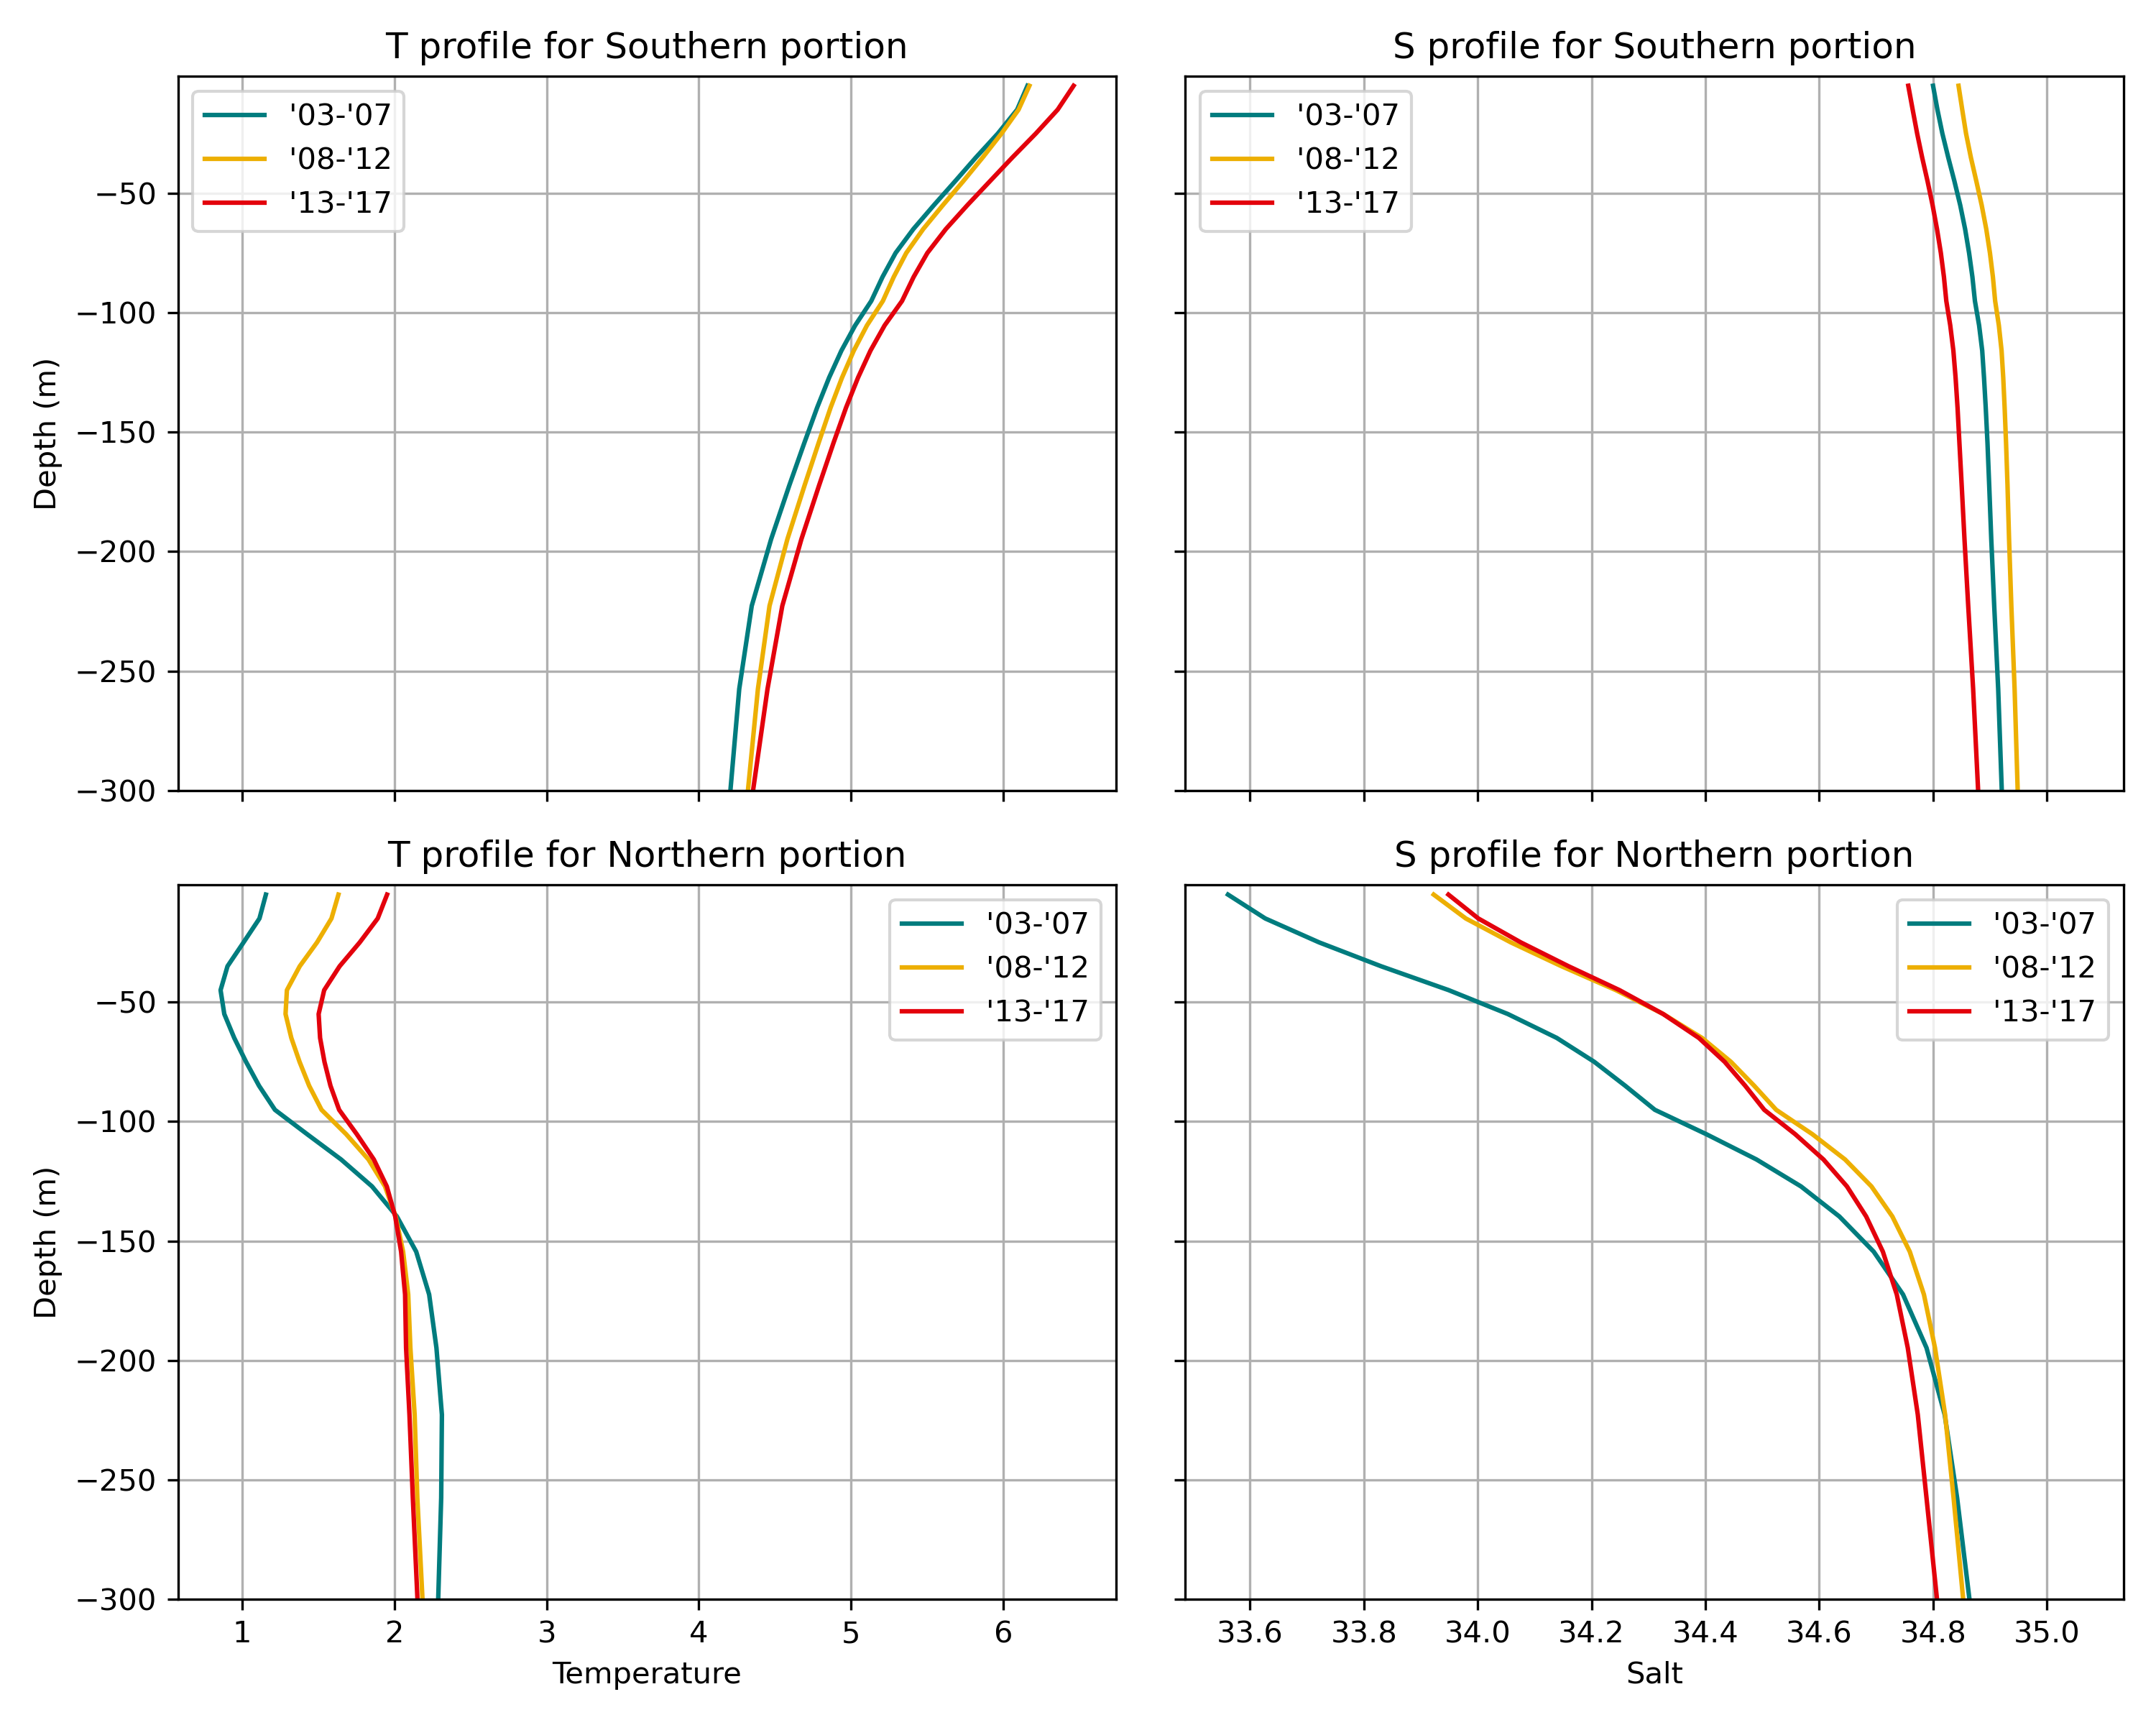
\includegraphics[width=\linewidth]{figs/profiles.png}
    \caption{\emph{T} and \emph{S} profiles show warming and salinification in the northern part of the Barents Sea, while the Southern part exhibits warming and freshening over the three time periods (2003–2007, 2008–2012, and 2013–2017).}
    \label{fig:profiles}
    \vspace{-30pt}
\end{wrapfigure}

% connecting the barents sea to the Arctic circulation
The Barents Sea serves as a transition zone between the Arctic and Atlantic Oceans. The sea is composed of several water masses, each defined by their temperature (\emph{T}) and salinity (\emph{S}). Warm, saline Atlantic Water (AW) and relatively, cold fresh Arctic Water (ArW) are the primary two externally-sourced water masses to the Barents Sea, in addition Norwegian Coastal Current Water (NCCW) \cite{Loeng1991,Smedsrud2010}. Local formation of meltwater and bottom water also contribute to the region's hydrography \cite{Oziel2016}. ArW is advected southward only to the Polar Front (PF), a key hydrographic feature of the region. In the western Barents Sea, the PF is steered by bathymetry, whereas in the east, the front broadens and splits into two distinct fronts characterized by sharp lateral gradients in temperature and salinity, respectively \cite{Oziel2016}. This boundary delineates where AW loses heat to the atmosphere and freshens from sea ice melt, precipitation, and runoff as well as it determines where AW is subducted beneath the ArW layer as modified Barents Sea Water (BSW) \cite{Oziel2016,Barton18}. This BSW continues to propagate northward before it enters the Arctic Basin primarily through the St. Anna Trough (Fig.~\ref{fig:map}) \cite{schauer2002}. Consequently, the PF effectively divides the Barents Sea into two distinct regimes. South of the PF, the Barents Sea is stratified by temperature and strongly influenced by AW inflow and atmospheric heat fluxes \cite{Hakkinen2009}. In contrast, the northern Barents Sea exhibits salinity-driven stratification (Figure~\ref{fig:profiles}), sustained by ice melt and more closely resembling the Arctic Ocean stratification \cite{kolas2024}. This salt-stratified northern regime is often referred to as a "beta" ocean \cite{Nansen1902,Carmack2007,Stewart2016}; contrasting this is the "alpha" ocean, which describes most of the global oceans and is primarily temperature-stratified. This two-regime system means that surface processes in the southern regime of the Barents Sea play a key role in preconditioning heat and salt transported to the central Arctic \cite{Parsons1996,Munk1998,Garrett2003,Vage2014,kolas2024}. However, recent Atlantification has increased the heat content in the Barents Sea, intensifying temperature gradients across the PF and limiting sea ice extent \cite{Barton18}. The cumulative changes to the Barents Sea--increased heat inflow, reduced sea ice extent, changing atmospheric conditions--have restricted the capacity for surface cooling to occur and meant warmer outflows to the Arctic \cite{Skagseth2020}.

\begin{wrapfigure}{r}{0.6\textwidth} % 'r' for right, '0.5\textwidth' for width
    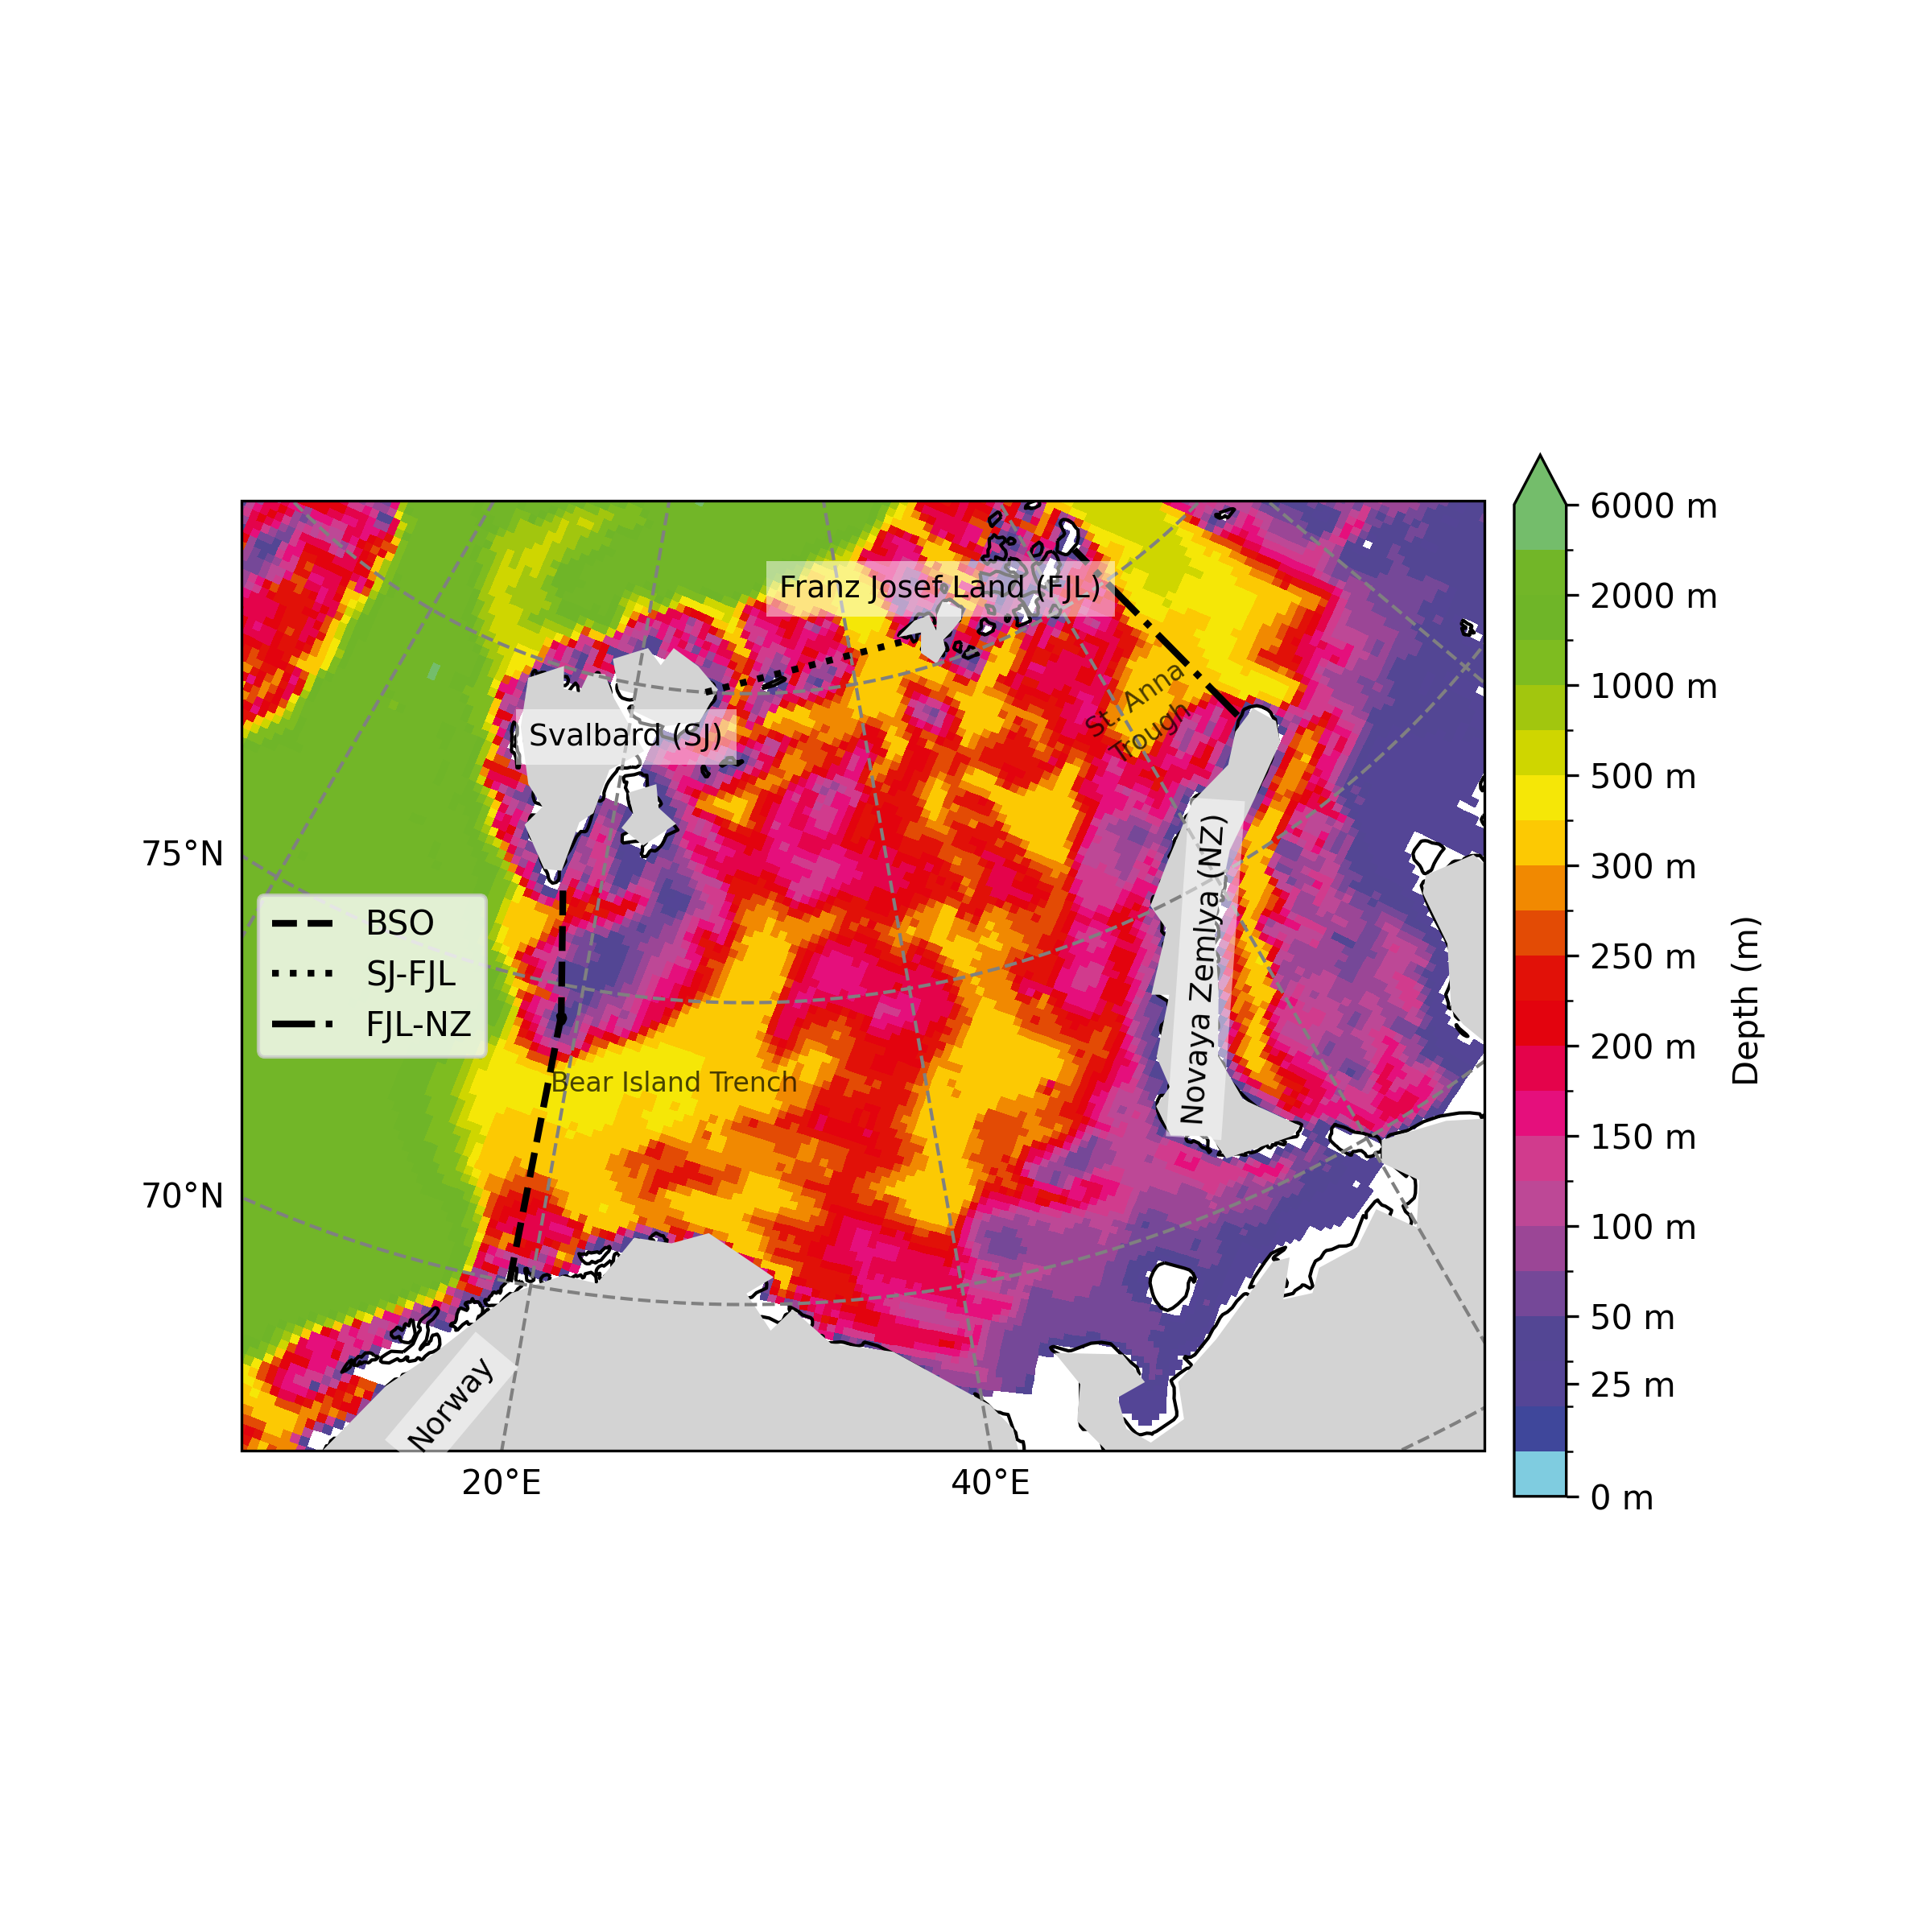
\includegraphics[width=\linewidth]{figs/BarentsS_Bathymetry.png}
    %\vspace{-100pt} % Adjust this value as needed to reduce space
    \caption{Bathymetry of the Barents Sea, highlighting variations on the continental shelf. The Barents Sea is a shallow continental shelf sea bounded by Svalbard (SJ) to the west, Franz Josef Land (FJL) to the north, Novaya Zemlya (NZ) to the east, and Norway to the south. Notable bathymetric features include the Bear Island Trench and the St. Anna Trough. Key gateways to the Sea are labeled as dashed lines.}
    \label{fig:map}
    \vspace{-25pt}
\end{wrapfigure}

% Arctic Ocean circulation- connecting the Barents Sea to the bigger picture
Barents Sea throughflow supplies half of the Atlantic-sourced water to the Arctic Ocean \cite{Lien_Trofimov_2013}. Transported at depth, this AW holds enough heat to melt Arctic sea ice were it hypothetically to reach the surface \cite{Polyakov2017,Stroeve2018,Grabon2021}. Upon entry to the AO, the Barents Sea branch of Atlantic-sourced water merges with another relatively warmer, saltier inflow branch arriving via the Fram Strait \cite{schauer1997,Lien_Trofimov_2013}. Together, these waters mix and spread Eastward as part of the Arctic Ocean Boundary current system \cite{schauer1997,Wang2020,Rudels2022}. In the subsurface AO, water from the boundary current recirculates through the Nansen, Amundsen, Makarov and Canada basins, influenced by these bathymetric features before rejoining the boundary current system \cite{Rudels2022}. This process redistributes heat and salt along the continental margins and throughout the AO. Double-diffusive convection, particularly in the form of layered thermohaline "staircases", plays a role in cooling AW in the basins of the AO by facilitating upward heat transfer, gradually weakening the halocline by warming the surface layers \cite{Timmermans2008,shibley2017spatial}. This process is driven by vertical temperature and salinity gradients, where both temperature and salinity increase with depth, creating conditions favorable for diffusive convection \cite{Rudels2008,polyakov2019}. Along the continental slope, where these staircases are weaker or absent \cite{shibley2017spatial}, turbulent vertical mixing is more dominant in the vertical redistribution of heat due to bed shear friction \cite{Rippeth2015,Polyakov2020,schulz2021}. Changes to freshwater input occurring both in the Barents Sea and the internal Arctic have contributed to the weakening of the the cold halocline layer necessary to suppress vertical mixing \cite{Fer2009}, particularly along the Eurasian shelf \cite{Pemberton2016,Polyakov2020,Metzner2020}. This weakening of the halocline layer allows more heat to reach the surface, potentially accelerating sea ice loss and altering AO stratification \cite{Polyakov2017,Polyakov2020}.

% the Barents Sea itself and the water masses there, what about the polar front


%This has implications for the stability of the Arctic Ocean stratification and the vertical distribution of heat, which could exacerbate ice loss and alter circulation patterns across the basin. 


%Understanding these dynamics is crucial for evaluating the broader impacts of Atlantification on the Arctic system.

% weakening cold halocline later : \cite{Polyakov2020,Metzner2020}.

% PF is typically defined by the Northern Front which is salinity (Oziel, Barton)

% \begin{wrapfigure}{r}{0.5\textwidth}
%     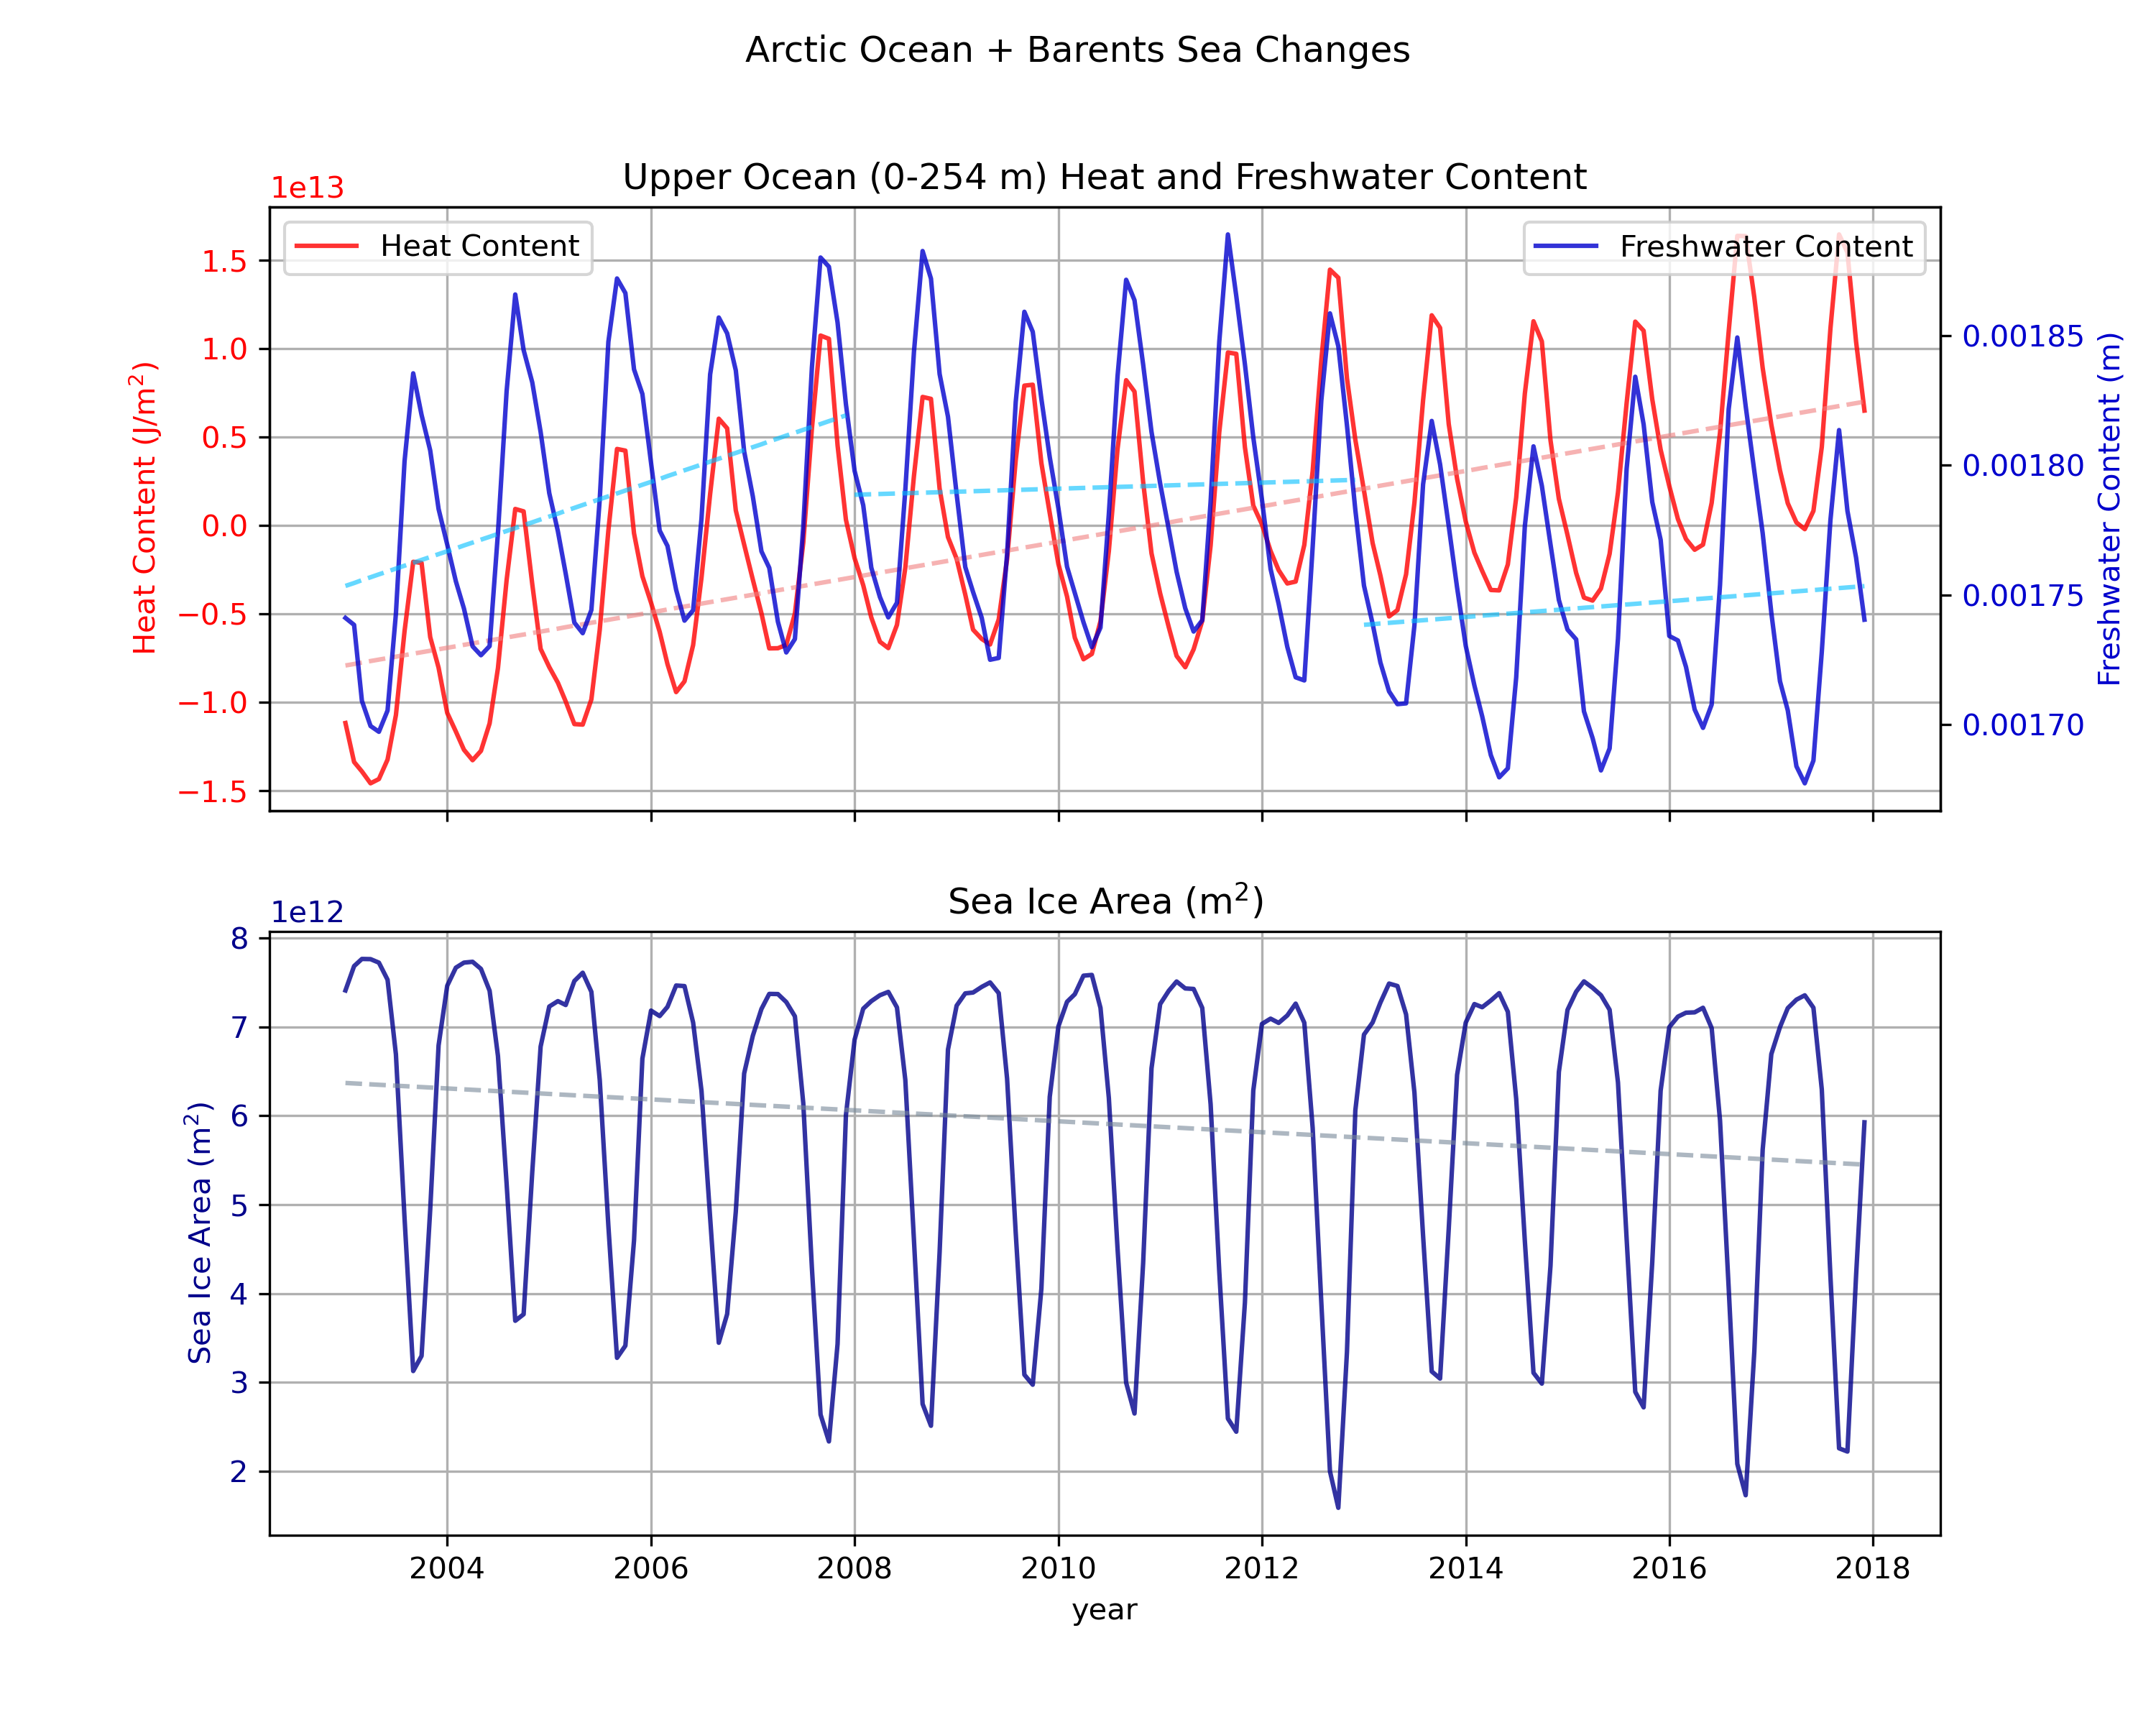
\includegraphics[width=\linewidth]{figs/Arctic_timeseries_proposal.png}
%     \caption{This is an example figure and caption that will be changed later...}
%     \label{fig:timeseries}
% \end{wrapfigure}

% fluid dynamics, geostrophic flow
% NOTE - should add some info about geostrophic flow
% NOTE - should also add some info on Ekman
% NOTE - should add some info about convection (vertical mixing due to density and thermal differences) and advection (horizontal transport of some tracer)
The large-scale dynamical impacts of Atlantification can be understood through the basic principles of ocean physics, which govern the redistribution of heat, salt and momentum. Heat and salt, directly tied to temperature (\emph{T}) and salinity (\emph{S}), are typically defined in oceanography as "active tracers", in that they influence turbulent flow \cite{Vallis2006}. Together with pressure, which increases with depth, these tracers determine the density of seawater, with colder, saltier water being denser than warmer, fresher water. Gravity plays a fundamental role in establishing and maintaining this density-driven stratification, as described by Archimedes' principle: a fluid parcel experiences an upward buoyant force proportional to the density difference with its surroundings, counteracting the downward pull of gravity. This balance creates a stable thermohaline stratification in the ocean in which denser layers lie below less dense ones, forming near-parallel isopycnal surfaces that extend across the ocean. To understand the behavior of isopycnals under Atlantification, we rely on both theoretical and numerical representations of hydrostatic balance. The general hydrostatic balance equation, which reflects the balance between buoyancy forces and pressure gradients, provides the conceptual framework, while the discretized form allows us to model these processes computationally. The general form of the hydrostatic balance can be written as:


\[
\frac{\partial p}{\partial z} = -\rho g
\]
where $\frac{\partial p}{\partial z}$ represents the vertical pressure gradient, $\rho$ is the local density of the fluid, and $g$ is the acceleration due to gravity. If the gravitational potential energy is expressed as:
$$
E = m g z
$$
where $m$ is mass, we can write the pressure gradient with geopotential $\Phi$ (the gravitational potential energy per unit mass) can be defined as:
$$
\Phi = \frac{E}{m} = gz
$$
We can then express the pressure gradient in terms of geopotential:
\[
\frac{\partial p}{\partial z} = -\rho \frac{\partial \Phi}{\partial z}
\]
Here, $\frac{\partial \Phi}{\partial z}$ is the vertical derivative of the geopotential, which equals $g$. This term represents the rate of change of gravitational potential energy per unit mass in the vertical direction and helps determine the vertical forces acting on the water, influencing any  vertical acceleration.

In the MITgcm, the vertical coordinate \(z\) are discretized into finite grid intervals \(\Delta z\). The derivative \(\frac{\partial \Phi}{\partial z}\) becomes a finite difference:

\[
\frac{\partial \Phi}{\partial z} = g \approx \frac{\delta_k \Phi_h'}{\Delta z}
\]
where $\delta_k \Phi_h'$ is the change in geopotential between adjacent grid points. Rewriting the general form of the hydrostatic balance, this becomes:


\[
\frac{1}{\Delta z} \delta_k \Phi_h' = g \rho
\]

In the MITgcm, the density is split into a reference density \(\rho_0\) and an anomaly \(\rho'\), such that \(\rho = \rho_0 + \rho'\), and the buoyancy term is $gp = g \overline{\rho'}^k$. The final local hydrostatic balance equation in discrete form is:

\[
\frac{1}{\Delta z} \delta_k \Phi_h' = g \overline{\rho'}^k
\]

This equation states that at each discrete grid level \(k\), the vertical pressure gradient force is balanced by the buoyancy force due to the density anomaly. In summary, hydrostatic equilibrium ensures that the geopotential gradient is balanced by local density anomalies. This balance maintains the vertical stratification of the ocean and acts to restore any local anomalies, ensuring that denser water remains below less dense water, thereby preserving ocean stability. When a water parcel is displaced vertically, the hydrostatic balance ensures that buoyancy forces act to adjust the parcel's position, restoring it to its equilibrium state and maintaining stratification.


% geostrophic flow
The uneven distribution of surface forcing--such as greater equatorial heating by shortwave radiation and spatially variable freshwater input--disrupts this stratification, creating horizontal and vertical density gradients. These gradients drive pressure differences which induce flow from regions of high to low pressure. However, Earth's rotation introduces Coriolis force, which deflects moving water to the right in the Northern Hemisphere and to the left in the Southern Hemisphere. The resulting geostrophic currents are thus a product of the pressure gradient ant the Coriolis force; in a steady state, this geostrophic balance leads to flow parallel to isopycnal surfaces rather than simply from high to low pressure. These currents are further developed by their interactions with topography and wind, which guide major global current systems, such as the North Atlantic Current. Geostrophic flow also facilitates meridional overturning, including the formation of bottom water. At high latitudes, water guided by geostrophic flow loses heat to the atmosphere, increasing its density and allowing it to sink, forming deep and bottom water as part of the global overturning circulation \cite{Vallis2006}. In the Arctic Ocean, geostrophic flow distributes heat from Atlantic and Pacific water, shelf processes provide external forcing that contributes to dense water formation and drives overturning \cite{Rudels2008}. To understand the evolution of an arbitrary tracer $\tau$--like heat or salt--in the ocean, we examine the balance of three terms in the advection-diffusion equation \cite{Campin2004}. Advection describes the transport of that tracer influenced by the velocity field and divergence, diffusion represents the smoothing of tracer gradients by redistributing tracers from high to low concentration, and external forcing which modifies tracer concentrations at the boundaries, such as surface fluxes. The changes to $\tau$ can be written through the following equation:

$$
\partial_t\tau + G^\tau_{adv} = G^\tau_{diff} + G^\tau_{forc}
$$

where
\begin{itemize}
    \item \(\tau\): The tracer concentration (e.g., temperature or salinity).
    \item \(\partial_t \tau\): The time rate of change of the tracer concentration.
    \item $(G^{\tau}_{adv})$: Advective tendency, describing the change in $\tau$ due to its transport by the velocity field.
    \item $(G^{\tau}_{diff})$: Diffusive tendency, describing the change in $\tau$ due to molecular or turbulent mixing smoothing the tracer gradients.
    \item $(G^{\tau}_{forc})$: The external forcing term, accounting for the addition or removal of the tracer by processes such as surface heating or freshwater input.
\end{itemize}

The advective tendency $(G^{\tau}_{adv})$ describes how $\tau$ is transported by the flow. This is written as:

$$
G^{\tau}_{{adv}} = \partial_x (u\tau) + \partial_y (v\tau) + \partial_z (w\tau) - \tau \nabla \cdot \mathbf{v}
$$

where

\begin{itemize}
    \item \(u, v, w\): The components of the velocity field in the \(x\), \(y\), and \(z\) directions, respectively.
    \item \(\partial_x (u\tau), \partial_y (v\tau), \partial_z (w\tau))\): the flux of the tracer in \(x\), \(y\), and \(z\), weighted by the velocity component.
    \item \(\nabla \cdot \mathbf{v}\): The divergence of velocity field, used to adjust for changes in tracer concentration at the surface where that tracer may be added.
\end{itemize}

The diffusive tendency term $(G^{\tau}_{{diff}})$ is written as:
$$
G^{\tau}_{{diff}} = \nabla \cdot (\mathbf{K} \nabla \tau)
$$

\begin{itemize}
    \item \(\mathbf{K}\): The diffusivity tensor, defining the rate of diffusion in each direction due to a gradient.
    \item \(\nabla \tau\): The gradient of the tracer, indicating how the tracer concentration changes in space.
    \item \(\nabla \cdot (\mathbf{K} \nabla \tau)\): The divergence of the tracer flux due to diffusion.
\end{itemize}

The diffusion term reduces tracer gradients by spreading the tracer from regions of high concentration to regions of low concentration. The use of the diffusivity tensor (\(\mathbf{K}\)) allows for the simulation of different diffusion rates in different directions, as occurs in stratified environments.

% how is this system disrupted - mixing
% eddy formation and baroclinic instability: Hunkins 1974 and Spall 1995
The relative roles of these three terms--advection, diffusion, and external forcing--in influencing the stable stratification of the ocean maintained by gravity and buoyancy are spatially variable. These processes influence where and how mixing can occur by creating the physical conditions necessary for different mixing mechanisms \cite{StoleHansen1991,Speer1993,long2017}. External forcing alters tracer concentrations at the surface and boundaries, while advection and diffusion work together to redistribute heat and salt, thereby modifying thermohaline stratification \cite{Munk1966}. Advection transports ocean properties along isopycnals, and can establish horizontal density gradients. For example, if warm salty AW is advected into a region with ArW, this can lead to isopycnal tilting, where horizontally, warm salty water is next to cold fresh water. This tilting is a potential energy reservoir; denser water is positioned horizontally next to lighter water. In the rotating ocean, this horizontal density gradient causes horizontal velocity to change with depth, creating vertical shear. This shear makes the system susceptible to perturbations, which can release stored potential energy energy. This process is the essence of baroclinic instability, the mechanism that converts potential energy stored in these gradients into kinetic energy, giving rise to the formation of mesoscale eddies \cite{Vallis2006}. These eddies play a pivotal role in diffusing heat and salt isopycnally, effectively homogenizing ocean properties and reducing the horizontal gradients of \emph{T} and \emph{S} between isopycnal surfaces. Velocity gradients induced by eddies can generate shear and small-scale turbulence, which can, in turn, lead to diapycnal (vertical) mixing \cite{Vallis2006}. This diapycnal mixing is particularly important at frontal zones with sharp lateral density gradients, such as the PF \cite{Oziel2016}. Thus, mesoscale eddies enable some degree of cross-frontal exchange, which can alter horizontal density gradients and weaken stratification \cite{kolas2024}. In addition to eddy diffusion, molecular diffusion acts diapycnally, transferring heat and salt across isopycnals from warmer to cooler and saltier to fresher regions, yet these effects are small compared to the larger-scale processes associated with mesoscale eddies \cite{Kagan2015}. Vertical turbulent mixing, which acts to transport properties across isopycnals, often requires external energy sources such as wind stress and tidal forcing. These forces generate turbulence and internal waves which induce vertical mixing. Additionally, buoyancy-driven processes, like double-diffusive mixing or convection, which occurs when stratification is unstable, can further enhance vertical mixing \cite{Vallis2006}. In the Barents Sea, the relative roles of these processes are shifting due to climate change. As the composition of inflowing AW shifts, so too are the gradients in \emph{T} and \emph{S}, enhancing potential vorticity (PV) gradients and limiting the expansion of sea ice across the PF \cite{Oziel2016,Barton18}. Increased wind stress over an increasingly ice-free ocean imparts momentum to the surface ocean, increasing vertical shear and further amplifying eddy activity \cite{Shao2023,li2024eddy}, enhancing the redistribution of ocean properties at the PF \cite{Porter2020}. Additionally, the retreat of sea ice enhances the influence of Atlantic heat on the surface ocean, further impacting sea ice \cite{Dorr2024}, highlighting the significance of ongoing changes in the region.

% i think this might be better served as a paragraph on how these things are changing
% some notes on turbulence -- might be a paragraph and might not

%DRAFT: tidal mixing and bed shear stresses
% another note - timmermans 2008 but this is for CAA - can we cite?
% The vertical mixing driven by turbulence which can act to reduce stratification is particularly important over rough topography
% Tidal mixing can be introduced as a source of energy that disrupts stratification and contributes to mixing near the seabed and in regions with strong density gradients, such as the PF.
% Bed shear stresses can be linked to turbulence generation near the seafloor, affecting the bottom boundary layer and facilitating vertical mixing.


% Cole 2015, 
% intro paragraph on WMT -- what it is and why do we care
% summarizee some insights provided by earlier studies on why the WMT framework is useful
One approach to quantify the changes in \emph{T} and \emph{S} is through the water mass transformation (WMT) framework \cite{Walin_1977,Walin1982}. Water masses, defined by distinct sets of \emph{T} and \emph{S} coordinates, have long been used to study the stratification and large scale circulation in the ocean because of their relation to ocean density \cite{sverdrup1942}. In this framework, a "transformation" describes the process by which one ocean water mass--defined by a volume enclosed between isothermal and isohaline surfaces--is converted into another through changes in \emph{T} and \emph{S}. These changes are driven by advection, internal diffusion, and external forcing.

\begin{figure}
    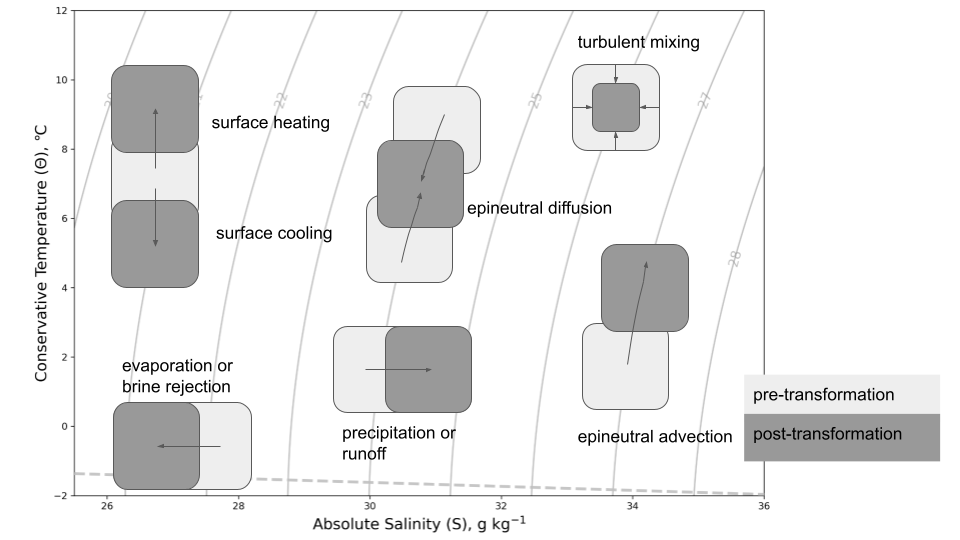
\includegraphics[width=\linewidth]{figs/TS_example.png}
    \vspace{-5pt} % Adjust this value as needed to reduce space
    \caption{This schematic illustrates potential modifications to temperature (\emph{T}) and salinity (\emph{S}) in the ocean through water mass transformation (WMT). Arrows indicate the direction and processes driving WMT, while shaded regions represent the volume distribution within \emph{T}--\emph{S} space. Epineutral action occurs along the density surfaces, shown as gray lines.}
    \label{fig:TS_example}
    \vspace{-20pt}
\end{figure}

% state of the art/history of literatutre
Substantial effort has been undertaken to develop a WMT framework for the ocean in tracer coordinates. By the conservation equations in tracer coordinates, \citeA{Walin_1977} and \citeA{Walin1982} demonstrated how water mass transformation and ocean circulation patterns can be inferred from surface fluxes and interior mixing. \citeA{Walin_1977} studied estuarine systems, and using salinity as a tracer, derived the relationship between volume transport across isohaline surfaces and salt forcing due to surface fluxes and mixing. In a subsequent paper, \citeA{Walin1982} applied temperature as a tracer, formulating volume and heat conservation relations to study the effects of advective and diffusive heat fluxes on the temperature distribution of the ocean. These two papers thus laid the foundation for descriptions of WMT in tracer--not geographic--coordinates, enabling water mass formation calculations from air-sea fluxes. \citeA{Speer1993} generalized the \citeA{Walin_1977, Walin1982} framework to use \emph{S} and \emph{T} coordinates simultaneously, using the continuity equations to show how the thermodynamic budgets for heat and freshwater can be used to describe WMT due to heat and freshwater fluxes. His work used a two-dimensional vector $(\mathbf{J})$ to describe the conversion rate of one water mass into another:

\[
\mathbf{J} = 
\left( \frac{\partial G_S}{\partial T}, \frac{\partial G_T}{\partial S} \right)
\]

Here, if $\partial G_S$ and $\partial G_T$ are the volume flows across isohaline and isothermal surfaces, respectively, a positive $\frac{\partial G_S}{\partial T}$ describes the transformation of water towards higher at the salinity $S$ in a particular temperature range, and $\frac{\partial G_T}{\partial S}$ gives a similar transformation of water towards higher temperatures at $T$ in a given salinity range.

The rate $\mathbf{J}$ describes the volume flux across isothermal or isohaline surfaces, with the volume of water between these layers as a water mass. At the outcrops of these thermohaline surfaces, surface forcing can add or remove salt or heat, pushing these surfaces outward or inward. Meanwhile, internal diffusion smooths tracer gradients across these boundaries, shifting the surfaces toward regions with weaker tracer concentrations. Advection, by the conservation of mass, cannot alter the total volume of a thermohaline layer but can deform or displace these surfaces. For instance, advection may shift the location of these surfaces horizontally or vertically, thereby strengthening or weakening stratification. Additionally, advection can modify horizontal gradients of \emph{T} and \emph{S}, which in turn affect the local exchange of heat and freshwater with the atmosphere. The transformation rates introduced by \citeA{Walin1982} quantify the shifts across these thermohaline surfaces as transformation rates; it is the divergence of these rates that indicate the net rate at which a water mass is formed or destroyed. This means that advection acts isopycnally by redistributing water properties, altering fluxes across the surface and influencing the accumulation or destruction of certain water masses \cite{Maze2009}. To synthesize these ideas into a broader framework, \citeA{doos2012} and \citeA{zika2012} introduced a time-averaged thermohaline streamfunction, intended to show that in a steady state, transformation vectors for the global ocean show no net-convergence. \citeA{Groeskamp2014} further developed the streamfunction to account for the instantaneous velocity and the movement of isohaline and isothermal surfaces in time. Interestingly, the global streamfunction is nonzero, in that volume transport across iso-surfaces does not fully converge or cancel out, particularly duruing periods of seasonal variability. \citeA{Groeskamp2014} demonstrates that seasonal variability accounts for some WMT that cannot be captured by a time-mean streamfunction alone. In other words, a time-varying approach with resolved surface fluxes is necessary to study the interannual and seasonal differences in the shifting isopycnal surfaces.

% establishing the use of \emph{T}--\emph{S} analysis as an approach to studying WMT and making it possible to calculate the convergence of any given water mass due to surface processes.

% the T--S framework
\emph{T}--\emph{S} analysis, formalized by \citeA{Hieronymus2014}, provides a powerful framework for understanding WMT. Developed from the original ideas of \citeA{Walin1982}, the \citeA{Hieronymus2014} framework formulated a continuity equation in \emph{T}--\emph{S} space, enabling the decomposition of WMT drivers into process-specific terms using a transformation vector. Building on the setup of \citeA{Speer1993}, \citeA{Hieronymus2014} incorporated isoneutral and dianeutral mixing, allowing for a breakdown of the influences on \emph{T} or \emph{S} independently. This breakdown of forcing terms was inspired from other studies which worked to quantify these processes using density alone \cite{Tziperman1986,Nurser1999,Marshall1999,Iudicone2008}, but the use of both \emph{T} or \emph{S} coordinates allows for a more nuanced representation of WMT. In this approach, traditional geographic coordinates (latitude, longitude, and depth) are translated into a two-dimensional \emph{T}--\emph{S} representation, allowing volumes of water within specific \emph{T} and \emph{S} ranges to be visualized. This framework is particularly effective for identifying water masses, analyzing their interactions, and studying mixing and circulation patterns on a process-based scale, rather than focusing solely on regional or basin-specific processes. \emph{T}--\emph{S} analysis is particularly beneficial in beta oceans, where analysis in \emph{T} or density alone would fail to account for surface freshwater influences on WMT. In the Arctic, \emph{T}--\emph{S} analysis helps to resolve both the impact of increased surface warming from AA and changes to freshwater forcing, providing a more comprehensive understanding of WMT and density changes.

% NEW PARAGRAPH: Pemberton; what they did, how it contributed to general understanding, what was the limitation (time period, time mean vs time varying), budget nonclosure, why new work is needed given the tools that currently exist
\citeA{Pemberton2015} used the framework developed by \citeA{Hieronymus2014} to analyze WMT in the Arctic Ocean, with a focus on the contributions from surface fluxes, mixing processes, and boundary exchanges through the Arctic gateways. Their objective was to determine whether the Arctic Ocean could be realistically represented within the WMT framework, particularly to identify which long-term processes transform AW and Pacific Water into Arctic outflow. Utilizing 26 years of output from a global ocean circulation model, \citeA{Pemberton2015} utilized a time-mean approach to study Arctic and regional WMT, including the Barents Sea. They assume a steady-state after the spin-up in which inflows, outflows and internal processes on average achieve quasi-equilibrium. This enabled them to identify the dominant processes impacting WMT in the Arctic. They found that surface heat fluxes play a dominant role in cooling Atlantic inflow, particularly in the Barents Sea, while vertical mixing and to a lesser extent surface freshwater fluxes act to decrease salinity near the freezing line before return flow to the North Atlantic. However, the reliance on time-mean--rather than time-varying--analysis precluded the effect of seasonal dynamics, short-term variability, and interannual changes on WMT \cite{Tsubouchi2018}. As a result, the seasonal variability of surface fluxes remains unresolved, a notable limitation given the role these processes play in AA and the transformation of inflowing waters. Furthermore, the 26-year period constrained their ability to capture the rapid changes to the Arctic, particularly regions like the Barents Sea, where short term variability in sea ice and heat fluxes play a key role in the properties of the sea. Time-varying analyses that account for the cumulative forcing terms and how these shape the Arctic system over both seasonal and interannual time scales are thus necessary. Additionally, if mass, heat and salt were conserved, WMT analysis would exhibit budget closure, in which any change in \emph{T} and \emph{S} is accounted for by their corresponding tendency terms. However, the budgets in \citeA{Pemberton2015} exhibit nonclosure, with discrepancies arising from the linear free-surface used in their model. While this method allowed them to resolve the largest contributors to heat and salt changes, more detailed processes of WMT, particularly in the salt budget, may have been excluded from their analysis. Building off the work of \citeA{Pemberton2015}, new analyses incorporating a time-varying approach to WMT is needed to provide a more comprehensive understanding of Arctic changes, for which closed budgets can be a useful tool.

% outline of the paper
Guided by previous work, we aim to quantify the relative contributions of surface fluxes, advection, and mixing to water mass transformations (WMT) in the Barents Sea and their seasonal and interannual variability. Using the WMT framework, we will identify the dominant processes driving the observed Atlantification of the Barents Sea. Additionally, we will explore how seasonal and interannual changes in surface forcing influence stratification and heat transport in the context of a changing climate.

%%%%%%%%%%%%%%%%%%%%%%%%%%%%%%%%%%%%%%%%%%%%%%%%%%%%%%%%%%%%%%%%%%%%%%%%%%%%%%%%%%%%%%%%
% Parking
% Because seawater density and stratification depend directly on these variables, understanding their distribution offers  valuable information on the circulation of the ocean.

% \citeA{Evans2023} used a similar framework to find that air-sea fluxes precondition the northward flow of AW, and mixing sets the properties of NADW in the Nordic Seas, but this study had large residuals. The importance of mixing in this study underscores the need to study what is generating this turbulent mixing.

% \cite{Hieronymus2014}: This further allowed for the attribution of WMT to specific processes, but did not include convection or bottom boundary terms, and thus did not close a budget. 

% \cite{Pemberton2015}: While this application provided valuable insights into dominant, long-term transformation trends, it did not close the budget nor address shorter-term processes, leaving gaps in understanding the relative impacts of various transformation mechanisms in Arctic WMT.

% \cite{Evans2023}: wmt with residuals


% % paragraph introducing/motivating WMT in the Barents Sea/how has this been applied in other studies
% As the heat and salinity of the Barents Sea change, so too does its buoyancy. Ocean stratification is determined by buoyancy---a crucial term in the vertical momentum equation. Positive buoyancy drives upward acceleration, while negative buoyancy causes downward motion, influencing the stability of the water column. In a stratified ocean, buoyancy depends on density, which acts to restore displaced fluid particles to maintain equilibrium. In seawater, fluid density ($\rho$) depends on temperature and salt, but salinity changes exert a far greater impact on $\rho$. This makes salinity an important factor shaping stratification, particularly in polar regions where surface salt fluxes are substantial.


% WMT in the Barents Sea -- what's the point
% We employ a fully-closed WMT framework in \emph{T}--\emph{S} space for the Barents Sea. Closed budgets, derived from continuity equations, are essential for accurately capturing heat and freshwater variability by accounting for all contributing terms. The elimination of residuals thus allows us to ascertain the attribution of both dominant and minor physical processes on \emph{T} and \emph{S} changes. In the context of Atlantification in the Barents Sea, this framework is particularly valuable as it connects the changes in \emph{T} and \emph{S} to variations in density. The advection of AW is expected to play an important role in the observed warming and salinification of the Barents Sea, particularly in the northern, salinity-stratified regime. Surface heat fluxes and sea ice retreat further modulate surface transformation, reinforcing changes in the water column. Internal mixing contributes to WMT, homogenizing the previous contributions from advection and surface processes. Ultimately, the closed-budget WMT framework provides a comprehensive and nuanced understanding of the processes driving regime shifts in the Barents Sea, shedding light on the interplay between these processes.


% motivation and research questions; key gaps in knowledge; goals of the paper as quantifying WMT, identifying key drivers, and understanding their implications on the Arctic system
% (DRAFT) We hypothesize that the relative roles of AW import and surface process changes can be quantified using a budgeted WMT framework.
%%%%%%%%%%%%%%%%%%%%%%%%%%%%%%%%%%%%%%%%%%%%%%%%%%%%%%%%%%%%%%%%%%%%%%%%%%%%%%%%%%%%%%%%

\section{Methodology}\label{methods}


\subsection{Model Description}

% What is ASTE and why are we using it
We employ the Arctic Subpolar gyre sTate Estimage (ASTE), a high-resolution, data constrained ocean-sea ice model derived from the Massachusetts Institute of Technology general circulation model (MITgcm). The MITgcm solves the primitive equations using re-scaled $z^*$ coordinates, a vertical coordinate system that adjusts for free-surface variations by redistributing grid spacing to preserve computational efficiency and accuracy, with a fully non-linear free surface, enabling precise simulation of oceanic and cryospheric dynamics \cite{campin2008}. The sea ice model in the MITgcm is dynamic-thermodynamic, in that it accounts for both the physical movement of ice due to forces like winds, currents, and interactions with ice floes, as well as energy exchanges with the ocean and atmosphere. This model builds upon the frameworks developed by \citeA{Menemenlis2005} and \citeA{Losch2010}, which provide the foundation for coupling ocean and sea ice dynamics, to accurately model the growth, melt, and transport of sea ice. In addition explicitly defined large-scale processes, ASTE includes paramaterizations which replace processes that are too small-scale or complex to be physically represented. The isopycnal mixing paramaterization, based on \citeA{Redi1982}, describes how tracers like \emph{T} and \emph{S} are mixed along isopycnals. Eddy-induced tracer transport paramaterization, introduced by \citeA{Gent1990}, models the effects of mesoscale eddies on tracer distributions. Instead of resolving these eddies directly, this parameterization approximates their impact as additional diffusion and advection, effectively redistributing heat, salt, and other tracers vertically and horizontally. It also employs the nonlocal K-Profile Parameterization (KPP) scheme of \citeA{Large1994}, which unifies several vertical mixing processes in the ocean. KPP accounts for mixing in the interior, influenced by shear instability and internal wave activity, and enhanced mixing in the surface boundary layer driven by buoyancy and momentum fluxes. This approach enables a physically consistent match between the surface boundary layer and the ocean interior, incorporating both local (gradient-driven) and nonlocal (bulk-driven) contributions to vertical mixing, which has been validated against observations \citeA{large1997}. Together, these parameterizations ensure that the model captures the physics of ocean and sea ice, providing a robust framework for studying Arctic and sub-Arctic dynamics.

% grid and BC and basics
ASTE uses a finite-volume discretization in the LLC-270 grid configuration, which transitions from a latitude-longitude grid at low latitudes to a polar-cap topology, offering a nominal resolution of $\frac{1}{3}^\circ$ This corresponds to nominal grid spacings of ~16 km in the Nordic Seas and ~14 km in the Arctic interior. The model domain spans the Atlantic north of 32.5$^\circ S$, the Arctic Ocean, and marginal seas, with 50 vertical layers ranging from ~10 m at the surface to 500 m at depth. Observational bathymetry is integrated using partial cells to enhance the accuracy of seafloor representation, crucial for simulating transport along ridges and through seafloor canyons. Boundary conditions are prescribed from the global ECCOv4r3 solution, which assimilates satellite and in-situ observations to ensure consistency with large-scale oceanographic constraints. Atmospheric forcing is applied using bulk formulae with inputs from the JRA-55 reanalysis. The representation of temperature and salinity in the model incorporates parameterizations for turbulent mixing and eddy-driven transport, ensuring these processes are realistically accounted for despite being unresolved at the model's grid scale \citeA{Nguyen2021}.

% constraints and the importance of budget closure
ASTE is constrained by over $10^9$ satellite and in-situ observations between 2002 and 2017, minimizing a cost function to align model outputs with real-world data. The state estimation employs the non-linear adjoint framework developed within the Estimating the Circulation and Climate of the Ocean (ECCO) consortium, based on the MITgcm \cite{marshall_1997}, to iteratively optimize input parameters and initial conditions while ensuring adherence to conservation laws. This rigorous approach enables the closure of budgets for heat, salt, mass, and momentum at the grid scale, meaning all sources, sinks, and transports of these quantities are explicitly accounted for in the model. Unlike other reanalysis products, ASTE ensures that no term is omitted or underestimated, providing a consistent and physically complete representation of oceanic processes that allows for detailed and reliable diagnostics of the system. Recent developments include water mass transformation diagnostics, updated from \citeA{abernathey_2016}, further allows analysis of surface forcing, ocean transports, and mixing processes in both georgaphic and \emph{T}--\emph{S} space. These developments have enabled the ability to diagnose WMT both online and offline with budget closure.

\subsection{The Adjoint Method}

% motivation for the adjoint method
% One purpose of this study is to attribute recently observed changes in ocean heat transport (OHT) through the BSO to past variations in surface wind, thermal, and freshwater forcing.
One purpose of this study is to attribute observed changes in a given oceanic property of interest to past variations in external forcing, such as surface wind, thermal, and freshwater fluxes. Here, attribution refers to identifying the specific dynamical processes responsible for identifiable changes in the system. This can be achieved through sensitivity analysis, a technique that determines how variations in input variables, such as surface forcing, influence a quantity of interest, such as oceanic heat transport (OHT) or volume flow through a gateway. The traditional approach to performing attribution in an ocean model involves running an ensemble of forward model simulations, where the system evolves forward in time based on the initial control variables with different perturbations to the surface forcing, and analyzing how these changes affect the quantity of interest. This process helps identify sensitivities--the gradients of the quantity of interest with respect to inputs--which show how the output responds to variations in those inputs. However, in a state-of-the-art ocean model such as the MITgcm, the vast number of possible perturbations makes it computational expensive and technically challenging to run and process a sufficiently large ensemble for comprehensive sensitivity analysis. Instead, we employ the adjoint method, which efficiently computes the sensitivity of our quantity of interest to all possible surface forcing inputs simultaneously. This approach eliminates the need to run a large ensemble of forward model simulations with different inputs, providing clear insights into the causal mechanisms of heat transport variation by propagating sensitivities backward through the model. The resulting sensitivity maps reveal how global perturbations in surface wind stress, heat flux, and freshwater flux across different regions influence a property of interest, as well as the timescales over which these influences occur.

% ocean heat transport through the BSO.

% what is the adjoint method
To better understand how the adjoint method achieves this, it is useful to outline how the technique works in the context of ocean modeling. The cost function, or objective function, represents a scalar quantity of interest. Examples include the strength of the Atlantic Meridional Overturning Circulation (AMOC) at a specific latitude \cite{Pillar2016,Smith2019} or volumetric throughflow through a specific gate \cite{Nguyen2020}. In this study, we define OHT through the BSO as our cost function. The adjoint method computes the gradients of the cost function with respect to model inputs (control variables) by leveraging the forward model and automatic differentiation (AD). AD applies the chain rule to the forward model to derive both the tangent linear model (TLM) and the adjoint model. For example, in a model run with two time steps, $t_1$ and $t_2$, the TLM computes the partial derivatives of the state at $t_2$ with respect to the state at $t_1$. This describes how small perturbations in the control variables propagate forward in time, which is mathematically represented by the Jacobian matrix containing these partial derivatives. To compute the gradient of the cost function, the adjoint model--derived through AD of the forward model--propagates sensitivities backward in time using the transpose of the Jacobian matrix. Essentially, this process starts with the gradient of the cost function at $t_2$ and propagates it back to $t_1$. The result is the gradient of the cost function with respect to the control variables, obtained in a single adjoint run. With more time steps, this backward propagation allows us to trace how sensitivities evolve over time, providing insight into the timescales of sensitivity and revealing how perturbations at different times influence the cost function. At each time step, the adjoint model calculates how small changes in the control variables (e.g., heat flux, wind stress) influence the final cost function. This produces sensitivity maps that illustrate the extent to which perturbations in specific regions and inputs impact the cost function. 

\section{Projects}

\subsection{Project 1: Investigating Causes of Heat Accumulation in the Barents Sea}

% FIGURE 4: for the 5 years; motivate this with figure 1 (SI extent timeseries)
% goal of this is to show that the advective term is changing over time as a contribution to heating and salting

% motivation
The broad aim of this first project is to investigate the changing WMT rates in the Barents Sea to identify the most important long-term tendencies driving the convergence of water masses in \emph{T}--\emph{S} space. Of particular interest is the seasonal variability of these transformations, which has not yet been studied in detail nor with the use of closed budgets. By resolving seasonal patterns and their drivers, this work seeks to provide a more comprehensive understanding of how dynamic processes such as surface fluxes, advection, and mixing contribute to water mass evolution throughout the year, filling a critical gap in our knowledge of WMT in this region.


% example diagnostics
Figure~\ref{fig:sample_wmt} illustrates the water mass transformation (WMT) tendencies in the Barents Sea for 2014, broken down into individual contributors: (A) Observed total tendency, (B) Advection tendency, (C) Diffusion tendency, (D) KPP mixing tendency, (E) Surface forcing tendency, and (F) Sum of all tendencies. Each panel represents transformations in temperature-salinity (\emph{T}--\emph{S}) space, with the background color indicating log-transformed volume ($\log_{10}$ of $m^3/^\circ$C/PSU), grouped into distinct water masses based on \emph{T} and \emph{S}. Overlaid quiver arrows depict the transformation rates for these water masses, with arrow lengths scaled to reflect magnitude. This decomposition provides a detailed view of how each contributing process contributes to changes in water mass properties.


    \begin{wrapfigure}{l}{0.8\textwidth} % 'r' for right, '0.5\textwidth' for width
    \centering
    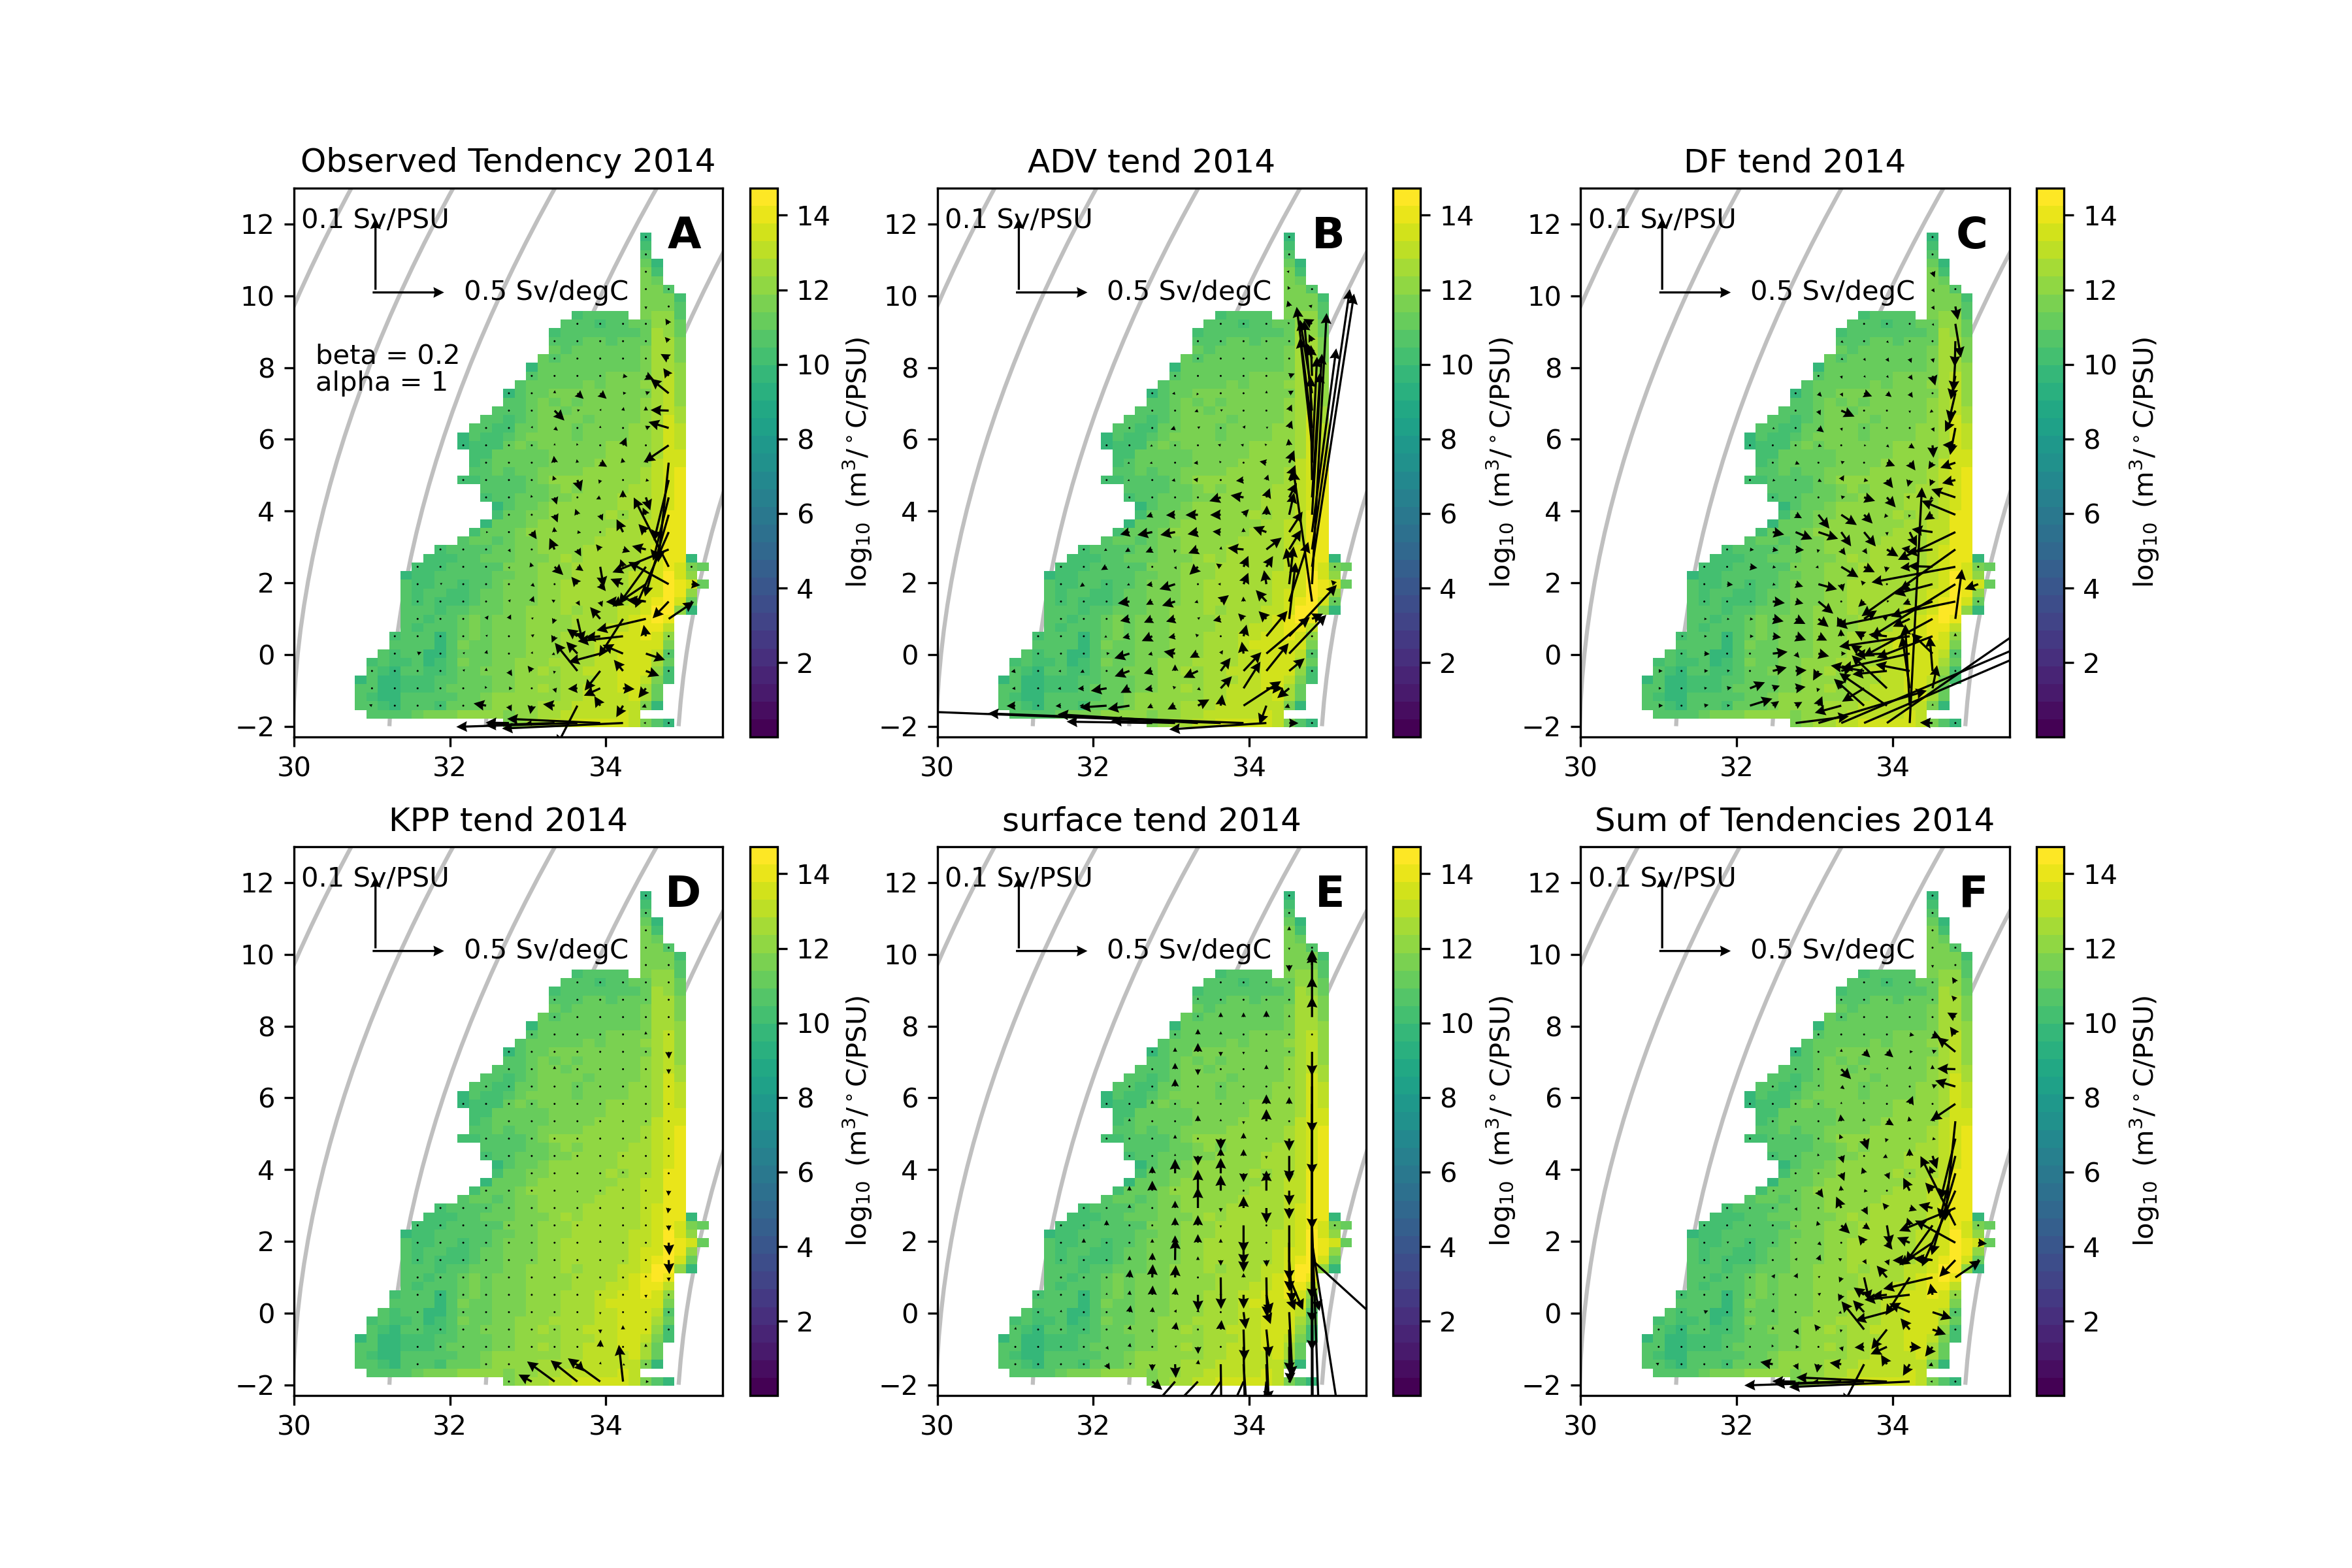
\includegraphics[width=\linewidth]{figs/BarentsS_alltend_2014.png}
    \caption{\emph{T}-\emph{S} diagrams from ASTE Release 1 for the year 2014 in the Barents Sea, showing the net transformation calculated from the change in \emph{T} and \emph{S} over time (A), which is broken down into components due to advective (B), diffusive (C), KPP (D), and surface (E) fluxes. The sum of B-E is shown in F, which is equivalent to A.}
    \label{fig:sample_wmt}
    \end{wrapfigure}

The total tendencies (Fig.~\ref{fig:sample_wmt}A) are derived from the rates of change in temperature ($\frac{dt}{dT}$) and salinity ($\frac{dt}{dS}$), normalized by the bin widths in \emph{T} and \emph{S}. Figure~\ref{fig:sample_wmt}B demonstrates that advective fluxes primarily increase the temperature and salinity of the Barents Sea, driven by the inflow of Atlantic Water (AW) through the Barents Sea Opening. Diffusive fluxes (Fig.\ref{fig:sample_wmt}C) act to homogenize water masses, redistributing cold, fresh water and warm, salty water towards intermediate values of \emph{T} and \emph{S}. Surface fluxes (Fig.\ref{fig:sample_wmt}E) predominantly transform Atlantic Water into cooler states, while KPP mixing (Fig.~\ref{fig:sample_wmt}D) operates along the freezing line, warming the water in this region. Finally, the combined tendencies (Fig.\ref{fig:sample_wmt}F) represent the sum of the individual contributions from advection, diffusion, surface fluxes, and KPP mixing (Figs.\ref{fig:sample_wmt}B--E). The absence of residuals in ASTE ensures that the total tendencies (Fig.~\ref{fig:sample_wmt}A) are perfectly reconstructed by this decomposition, confirming the conservation of heat and salt in the model.

% accumulation and why is convergence important
In the WMT framework, the convergence or divergence of transformation vectors represents the accumulation or destruction of water masses, respectively. Over an averaged time period, we can thus investigate the net effects of each tendency to assess how each mechanism impacts the long-term distribution of water masses. Understanding the mechanisms and impacts of AW accumulation provides insights into broader processes such as heat transport to the Arctic, freshwater storage, and the potential for feedbacks that amplify polar amplification.  Furthermore, convergence can show how heat and salt are stored and redistributed in the sea. Beyond a single year or time period, examining persistent trends in convergence can elucidate long-term dynamical changes to this region, when the cumulative effects of transformation may be obscured by short-term variability. For example, in the Barents Sea, studying the sustained accumulation of AW allows us to evaluate how consistent tendencies influence Atlantification. Over longer time scales, WMT analysis reveals to what extent the Barents Sea is reaching a new Atlantic-like equilibrium or undergoing continual changes.

\subsection{Project 2: Broader Impacts on the Eastern Arctic}

% motivation and structure
The goal of this second project is to investigate changes in ocean heat transport (OHT) and vertical mixing in the Eastern Arctic through the WMT framework, focusing on their evolution over time and their contribution to Arctic stratification. The Eurasian Basin is typically covered with sea ice year-round, and melting occurs primarily from solar radiation at the surface. However, the extent and thickness of this ice have been declining in recent decades due to warming and increased solar radiation during summer. River runoff from Siberia and melting sea ice contribute freshwater to the surface, enhancing the stratification that maintains the halocline. The halocline, characterized by a sharp increase in salinity with depth while temperatures remain near freezing, is primarily sustained by the lateral advection of dense, saline water formed on the Arctic shelves during winter freezing and brine rejection \cite{aagaard1981}. This maintains the beta ocean structure of this region, wherein a surface mixed layer (SML) overlies the halocline, overlies a layer of AW and deep basin waters. The halocline largely shields the Arctic ice cover by limiting upward heat flux from the Atlantic layer as it propagates along the continental shelf of the East Arctic. Conversely, it serves as a heat sink for the Atlantic Water, contributing to its cooling and freshening \cite{aagaard1981}. Until recently, AW heat was not considered as a major factor for sea ice melt, but recent studies suggest it is an important heat source for vertical mixing induced melt \cite{Carmack2007,Polyakov2017}.


% structure of the East Arctic and how it is changing
Atlantification and the Eastern Arctic
The stratification of the Eastern Arctic is 

Building on the foundational work of
\citeA{Polyakov2017,polyakov2019,Polyakov2020}, which highlighted the critical role of Atlantic Water in warming the Arctic Ocean and weakening the halocline, this study aims to quantify the processes driving these changes. 

Polyakov's findings on the interplay between double-diffusive convection, turbulent mixing, and the redistribution of Atlantic heat provide a compelling framework for examining how vertical heat transport influences surface conditions and ice melt. By analyzing both long-term trends and seasonal variability, this project seeks to disentangle the relative contributions of OHT and vertical mixing to the observed Atlantification of the Eastern Arctic, providing new insights into the mechanisms shaping the region's response to a changing climate.

% return to the goal of this project - what are we trying to do

\subsection{Project 3: Dynamical Attribution to Ocean Heat Transport Through the BSO}

% purpose of this project
The third project will build upon the previous two projects to study attribution to heat OHT through the BSO.

The BSO is an important site for heat transport to the Arctic Ocean. The purpose of the third and final project will be to attribute OHT through the BSO to past variations in surface wind, thermal, and freshwater forcing. To do this, we will utilize the adjoint method to.

\section{Work plan}
    The Ph.D. program was started in Fall 2023. Anticipating the defense in Fall 2027 and taking  the degree timeline will resemble the following:

    \begin{enumerate}
        \item \textbf{Coursework, literature review, and preparing budgeting scripts:} Fall 2023 -- Spring 2024

        Deliverable: Python scripts to perform budget analysis in ASTE
        
        \item \textbf{Project 1:} Fall 2024 -- Spring 2025
        
        Deliverable: publication on the configuration of budget analysis tools to study changes to the Barents Sea, with a focus on heat content changes
        
        \item \textbf{Project 2:} Spring 2025 -- Summer 2026

        Deliverable: publication synthesizing the influence of internal mixing versus surface forcing on the changes to the Arctic Ocean heat transport 

        \item \textbf{Project 3:} Summer 2026 -- Summer 2027

        Deliverable: publication on adjoint sensitivity to synthesize the impacts of atmospheric variability on OHT through the BSO

        \item \textbf{Ph.D. Thesis:} Fall 2027

        Deliverable: Thesis
    \end{enumerate}

% FIGURE 5: highlight the convergence anomalies for the five years; compare this to figure 2 with the vertical stratification (redistribution away from the center to make a more average looking profile)
% focus on the one month (march) or maybe take a winter average motivated by the literature, use this for 2012 and 2014 to show that less sea ice -- less stratification -- redistribution of water away from the mixing line


%%

%  Numbered lines in equations:
%  To add line numbers to lines in equations,
%  \begin{linenomath*}
%  \begin{equation}
%  \end{equation}
%  \end{linenomath*}



%% Enter Figures and Tables near as possible to where they are first mentioned:
%
% DO NOT USE \psfrag or \subfigure commands.
%
% Figure captions go below the figure.
% Acronyms used in figure captions will be spelled out in the final, published version.

% Table titles go above tables;  other caption information
%  should be placed in last line of the table, using
% \multicolumn2l{$^a$ This is a table note.}
% NOTE that there is no difference between table caption and table heading in the final, published version
%
%----------------
% EXAMPLE FIGURES
%
% \begin{figure}
% \includegraphics{example.png}
% \caption{caption}
% \end{figure}
%
% Giving latex a width will help it to scale the figure properly. A simple trick is to use \textwidth. Try this if large figures run off the side of the page.
% \begin{figure}
% \noindent\includegraphics[width=\textwidth]{anothersample.png}
%\caption{caption}
%\label{pngfiguresample}
%\end{figure}
%
%
% If you get an error about an unknown bounding box, try specifying the width and height of the figure with the natwidth and natheight options. This is common when trying to add a PDF figure without pdflatex.
% \begin{figure}
% \noindent\includegraphics[natwidth=800px,natheight=600px]{samplefigure.pdf}
%\caption{caption}
%\label{pdffiguresample}
%\end{figure}
%
%
% PDFLatex does not seem to be able to process EPS figures. You may want to try the epstopdf package.
%

%
% ---------------
% EXAMPLE TABLE
%
% \begin{table}
% \caption{Time of the Transition Between Phase 1 and Phase 2$^{a}$}
% \centering
% \begin{tabular}{l c}
% \hline
%  Run  & Time (min)  \\
% \hline
%   $l1$  & 260   \\
%   $l2$  & 300   \\
%   $l3$  & 340   \\
%   $h1$  & 270   \\
%   $h2$  & 250   \\
%   $h3$  & 380   \\
%   $r1$  & 370   \\
%   $r2$  & 390   \\
% \hline
% \multicolumn{2}{l}{$^{a}$Footnote text here.}
% \end{tabular}
% \end{table}

%%%%%%%%%%%%%%%%%%%%%%%%%%%%%%%%%%%%%%%%%%%%%%%
% SIDEWAYS FIGURES and TABLES
% AGU prefers the use of {sidewaystable} over {landscapetable} as it causes fewer problems.
%
% \begin{sidewaysfigure}
% \includegraphics[width=20pc]{figsamp}
% \caption{caption here}
% \label{newfig}
% \end{sidewaysfigure}
%
%  \begin{sidewaystable}
%  \caption{Caption here}
% \label{tab:signif_gap_clos}
%  \begin{tabular}{ccc}
% one&two&three\\
% four&five&six
%  \end{tabular}
%  \end{sidewaystable}

%% If using numbered lines, please surround equations with \begin{linenomath*}...\end{linenomath*}
%\begin{linenomath*}
%\begin{equation}
%y|{f} \sim g(m, \sigma),
%\end{equation}
%\end{linenomath*}

%%% End of body of article

%%%%%%%%%%%%%%%%%%%%%%%%%%%%%%%%%%%%%%%%%%%%%%%
%% Optional Appendices go here
%
% The \appendix command resets counters and redefines section heads
%
% After typing \appendix
%
%\section{Here Is Appendix Title}
% will show
% A: Here Is Appendix Title
%
%\appendix
%\section{Here is a sample appendix}

%%%%%%%%%%%%%%%%%%%%%%%%%%%%%%%%%%%%%%%%%%%%%%%
% Optional Glossary, Notation or Acronym section goes here:
%
% Glossary is only allowed in Reviews of Geophysics
%  \begin{glossary}
%  \term{Term}
%   Term Definition here
%  \term{Term}
%   Term Definition here
%  \term{Term}
%   Term Definition here
%  \end{glossary}


%%%%%%%%%%%%%%%%%%%%%%%%%%%%%%%%%%%%%%%%%%%%%%%
% Acronyms
%% NOTE that acronyms in the final published version will be spelled out when used in figure captions.
%   \begin{acronyms}
%   \acro{Acronym}
%   Definition here
%   \acro{EMOS}
%   Ensemble model output statistics
%   \acro{ECMWF}
%   Centre for Medium-Range Weather Forecasts
%   \end{acronyms}


%%%%%%%%%%%%%%%%%%%%%%%%%%%%%%%%%%%%%%%%%%%%%%%
% Notation
%   \begin{notation}
%   \notation{$a+b$} Notation Definition here
%   \notation{$e=mc^2$}
%   Equation in German-born physicist Albert Einstein's theory of special
%  relativity that showed that the increased relativistic mass ($m$) of a
%  body comes from the energy of motion of the body—that is, its kinetic
%  energy ($E$)—divided by the speed of light squared ($c^2$).
%   \end{notation}




%%%%%%%%%%%%%%%%%%%%%%%%%%%%%%%%%%%%%%%%%%%%%%%
%
% DATA SECTION and ACKNOWLEDGMENTS
%
%%%%%%%%%%%%%%%%%%%%%%%%%%%%%%%%%%%%%%%%%%%%%%%

\section*{Open Research Section}
The ASTE\_R1 model configuration, inputs, and monthly and daily outputs are available at the Arctic Data Center (https://arcticdata.io).


\acknowledgments
Enter acknowledgments here. This section is to acknowledge funding, thank colleagues, enter any secondary affiliations, and so on.


%%%%%%%%%%%%%%%%%%%%%%%%%%%%%%%%%%%%%%%%%%%%%%%
% REFERENCES and BIBLIOGRAPHY
%
\bibliography{agusample} %don't specify the file extension
% don't specify bibliographystyle
%
%%%%%%%%%%%%%%%%%%%%%%%%%%%%%%%%%%%%%%%%%%%%%%%

%\bibliography{ enter your bibtex bibliography filename here }



%Reference citation instructions and examples:
%
% Please use ONLY \cite and \citeA for reference citations.
% \cite for parenthetical references
% ...as shown in recent studies (Simpson et al., 2019)
% \citeA for in-text citations
% ...Simpson et al. (2019) have shown...
%
%
%...as shown by \citeA{jskilby}.
%...as shown by \citeA{lewin76}, \citeA{carson86}, \citeA{bartoldy02}, and \citeA{rinaldi03}.
%...has been shown \cite{jskilbye}.
%...has been shown \cite{lewin76,carson86,bartoldy02,rinaldi03}.
%... \cite <i.e.>[]{lewin76,carson86,bartoldy02,rinaldi03}.
%...has been shown by \cite <e.g.,>[and others]{lewin76}.
%
% apacite uses < > for prenotes and [ ] for postnotes
% DO NOT use other cite commands (e.g., \citet, \citep, \citeyear, \nocite, \citealp, etc.).
%



\end{document}



More Information and Advice:

%%%%%%%%%%%%%%%%%%%%%%%%%%%%%%%%%%%%%%%%%%%%%%%
%
%  SECTION HEADS
%
%%%%%%%%%%%%%%%%%%%%%%%%%%%%%%%%%%%%%%%%%%%%%%%

% Capitalize the first letter of each word (except for
% prepositions, conjunctions, and articles that are
% three or fewer letters).

% AGU follows standard outline style; therefore, there cannot be a section 1 without
% a section 2, or a section 2.3.1 without a section 2.3.2.
% Please make sure your section numbers are balanced.
% ---------------
% Level 1 head
%
% Use the \section{} command to identify level 1 heads;
% type the appropriate head wording between the curly
% brackets, as shown below.
%
%An example:
%\section{Level 1 Head: Introduction}
%
% ---------------
% Level 2 head
%
% Use the \subsection{} command to identify level 2 heads.
%An example:
%\subsection{Level 2 Head}
%
% ---------------
% Level 3 head
%
% Use the \subsubsection{} command to identify level 3 heads
%An example:
%\subsubsection{Level 3 Head}
%
%---------------
% Level 4 head
%
% Use the \subsubsubsection{} command to identify level 3 heads
% An example:
%\subsubsubsection{Level 4 Head} An example.
%
%%%%%%%%%%%%%%%%%%%%%%%%%%%%%%%%%%%%%%%%%%%%%%%
%
%  IN-TEXT LISTS
%
%%%%%%%%%%%%%%%%%%%%%%%%%%%%%%%%%%%%%%%%%%%%%%%
%
% Do not use bulleted lists; enumerated lists are okay.
% \begin{enumerate}
% \item
% \item
% \item
% \end{enumerate}
%
%%%%%%%%%%%%%%%%%%%%%%%%%%%%%%%%%%%%%%%%%%%%%%%
%
%  EQUATIONS
%
%%%%%%%%%%%%%%%%%%%%%%%%%%%%%%%%%%%%%%%%%%%%%%%

% Single-line equations are centered.
% Equation arrays will appear left-aligned.

Math coded inside display math mode \[ ...\]
 will not be numbered, e.g.,:
 \[ x^2=y^2 + z^2\]

 Math coded inside \begin{equation} and \end{equation} will
 be automatically numbered, e.g.,:
 \begin{equation}
 x^2=y^2 + z^2
 \end{equation}


% To create multiline equations, use the
% \begin{eqnarray} and \end{eqnarray} environment
% as demonstrated below.
\begin{eqnarray}
  x_{1} & = & (x - x_{0}) \cos \Theta \nonumber \\
        && + (y - y_{0}) \sin \Theta  \nonumber \\
  y_{1} & = & -(x - x_{0}) \sin \Theta \nonumber \\
        && + (y - y_{0}) \cos \Theta.
\end{eqnarray}

%If you don't want an equation number, use the star form:
%\begin{eqnarray*}...\end{eqnarray*}

% Break each line at a sign of operation
% (+, -, etc.) if possible, with the sign of operation
% on the new line.

% Indent second and subsequent lines to align with
% the first character following the equal sign on the
% first line.

% Use an \hspace{} command to insert horizontal space
% into your equation if necessary. Place an appropriate
% unit of measure between the curly braces, e.g.
% \hspace{1in}; you may have to experiment to achieve
% the correct amount of space.


%%%%%%%%%%%%%%%%%%%%%%%%%%%%%%%%%%%%%%%%%%%%%%%
%
%  EQUATION NUMBERING: COUNTER
%
%%%%%%%%%%%%%%%%%%%%%%%%%%%%%%%%%%%%%%%%%%%%%%%

% You may change equation numbering by resetting
% the equation counter or by explicitly numbering
% an equation.

% To explicitly number an equation, type \eqnum{}
% (with the desired number between the brackets)
% after the \begin{equation} or \begin{eqnarray}
% command.  The \eqnum{} command will affect only
% the equation it appears with; LaTeX will number
% any equations appearing later in the manuscript
% according to the equation counter.
%

% If you have a multiline equation that needs only
% one equation number, use a \nonumber command in
% front of the double backslashes (\\) as shown in
% the multiline equation above.

% If you are using line numbers, remember to surround
% equations with \begin{linenomath*}...\end{linenomath*}

%  To add line numbers to lines in equations:
%  \begin{linenomath*}
%  \begin{equation}
%  \end{equation}
%  \end{linenomath*}



